%\documentclass[handout, 8pt]{beamer}
\documentclass[8pt]{beamer}

%\usetheme{Singapore}
%\usefonttheme{serif} 


%%%%%%%%%%%%%%%%%%%%%%%%
% Usual LaTeX Packages %
%%%%%%%%%%%%%%%%%%%%%%%%
\usepackage{pdfpages}
\usepackage{amsmath}
\usepackage{amscd}
\usepackage{amsfonts}
\usepackage{amssymb}
\usepackage{graphicx}
\usepackage{mathrsfs} 			% For Weinberg-esque letters
\usepackage{cancel}				% For "SUSY-breaking" symbol
\usepackage{slashed}            % for slashed characters in math mode
\usepackage{bbm}                % for \mathbbm{1} (unit matrix)
\usepackage{dsfont}
\usepackage{amsthm}				% For theorem environment
\usepackage{multirow}			% For multi row cells in table
\usepackage{arydshln} 			% For dashed lines in arrays and tables
\usepackage{multirow}
\usepackage{multicol}
\usepackage{bigstrut}
\usepackage{setspace}
\usepackage{endnotes}
\usepackage{etex}
\usepackage{lmodern}
\usepackage{booktabs}
\usepackage{graphics}
\usepackage[flushleft]{threeparttable}
%\usepackage{enumitem}
%\setlist[itemize]{itemsep=2mm}
\usepackage{array}
\usepackage{color}
\usepackage{colortbl}
\usepackage{hyperref}
\usepackage{ifplatform}
\usepackage{dcolumn}
\usepackage{threeparttable}
\usepackage{hyperref}
\usepackage{tabularx}
\usepackage{soul}
\usepackage{ulem}

\usepackage[utf8]{inputenc}
\usepackage[T1]{fontenc}
\usepackage{appendixnumberbeamer}
\usepackage{xcolor}
\def\boxit#1{%
  \smash{\color{red}\fboxrule=1pt\relax\fboxsep=2pt\relax%
  \llap{\rlap{\fbox{\vphantom{0}\makebox[#1]{}}}~}}\ignorespaces
}
\usepackage{appendixnumberbeamer}

\newcommand{\E}{\mathbb{E}}

% Code for Hiding Columns in Tables
\newcolumntype{H}{>{\setbox0=\hbox\bgroup}c<{\egroup}@{}}


\graphicspath{{images/}}	% Put all images in this directory. Avoids clutter.





% BIBLIOGRAPHY (OPTION: BIBLATEX) ===========================================
\usepackage{csquotes}
\usepackage[natbib = true, backend = biber, style  = authoryear-icomp]{biblatex}
\addbibresource{References.bib}

\usepackage{setspace}
\setbeamercovered{transparent}

%gets rid of navigation symbols
\setbeamertemplate{navigation symbols}{}

\setbeameroption{show notes}
%\setbeameroption{show only notes}
%\setbeameroption{hide notes}

% A simple slide counter at the bottom of the slide
\setbeamertemplate{footline}{
   \begin{beamercolorbox}[ht=4ex,leftskip=0.3cm,rightskip=0.3cm]{author in head/foot}
    \vspace{0.1cm}
    \hfill \insertframenumber / \inserttotalframenumber
  \end{beamercolorbox}
   \vspace*{0.1cm}
} 

\newcommand\independent{\protect\mathpalette{\protect\independenT}{\perp}}
\def\independenT#1#2{\mathrel{\rlap{$#1#2$}\mkern2mu{#1#2}}}




\title{The Controlled Choice Design and Paternalism in Pawnshop Borrowing}
\author{Craig McIntosh\inst{1} \and Isaac Meza\inst{2} \and Joyce Sadka\inst{3} \and Enrique Seira\inst{4} \and Francis J. DiTraglia\inst{5} }
\institute[UTran]{\inst{1} UCSD, \inst{2} Harvard , \inst{3} ITAM , \inst{4} MSU , \inst{5} Oxford} 
                      
\date{April 2023}

%\setbeamercolor{section in head/foot}{bg=darkcrimsonred}
\setbeamersize{text margin left=11pt, text margin right=11pt}
%\setbeamertemplate{section in toc}[square]




%%%%%%%%%%%%%%%%%%%%%%%%%%%%%%%%%%%%%%%
%%%%%%%%%%%%%%%%%%%%%%%%%%%%%%%%%%%%%%

\begin{document}


\begin{frame}[c, noframenumbering]%{\phantom{title page}}
% The \phantom{title page} is a kludge to get the red bar on top
\titlepage
\end{frame}


\section{Motivation}



\begin{frame}{Motivation: Private paternalism}
\begin{itemize}
    \vfill \item Many institutions —firms, schools, financial contracts— restrict choice using built-in commitment mechanisms which help workers, students, borrowers overcome self-control problems
    \begin{itemize}
        \item Loans with fixed repayment schemes, homework due dates, etc.
    \end{itemize}
    \vfill \pause\item At the same time these firms hide these forcing mechanisms and don’t market their commitment features, potentially because demand for them is low.
    \vfill  \item  Laibson (2018) argues that clients that benefit from commitment may underestimate its value, and that in such cases private paternalism (i.e. allocating them to commitment) could be beneficial.
    \vfill  \pause\item  \textbf{We study the (a) benefits of imposing a structured repayment contract on financing cost, (b) whether there is demand for such structure, and (c) whether non-takers of such a commitment product would benefit from taking it.}
\end{itemize}

\end{frame}



\section{Context}


\begin{frame}{Context}
\begin{columns}
\begin{column}{.45\textwidth}
\begin{figure}[H]
    \begin{center}
    \caption{Pawnshop}
        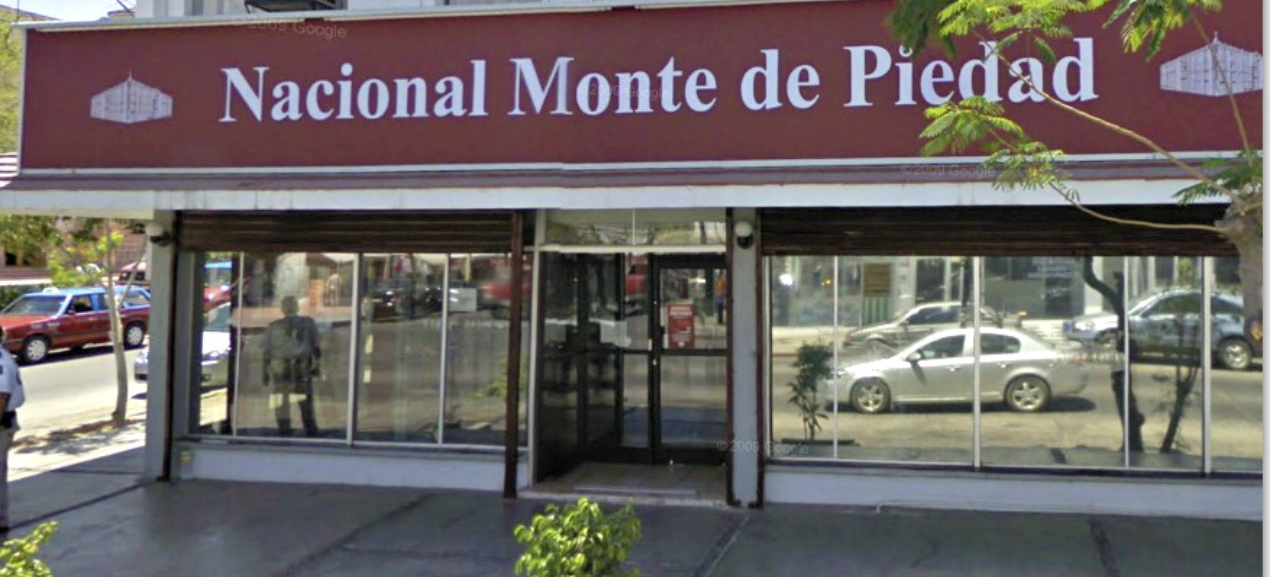
\includegraphics[width=0.95\textwidth]{Figuras/empenio2.png}
    \end{center}
    \end{figure}
\begin{figure}[H]
    \begin{center}
    \caption{Appraisers  inside a pawnshop}
        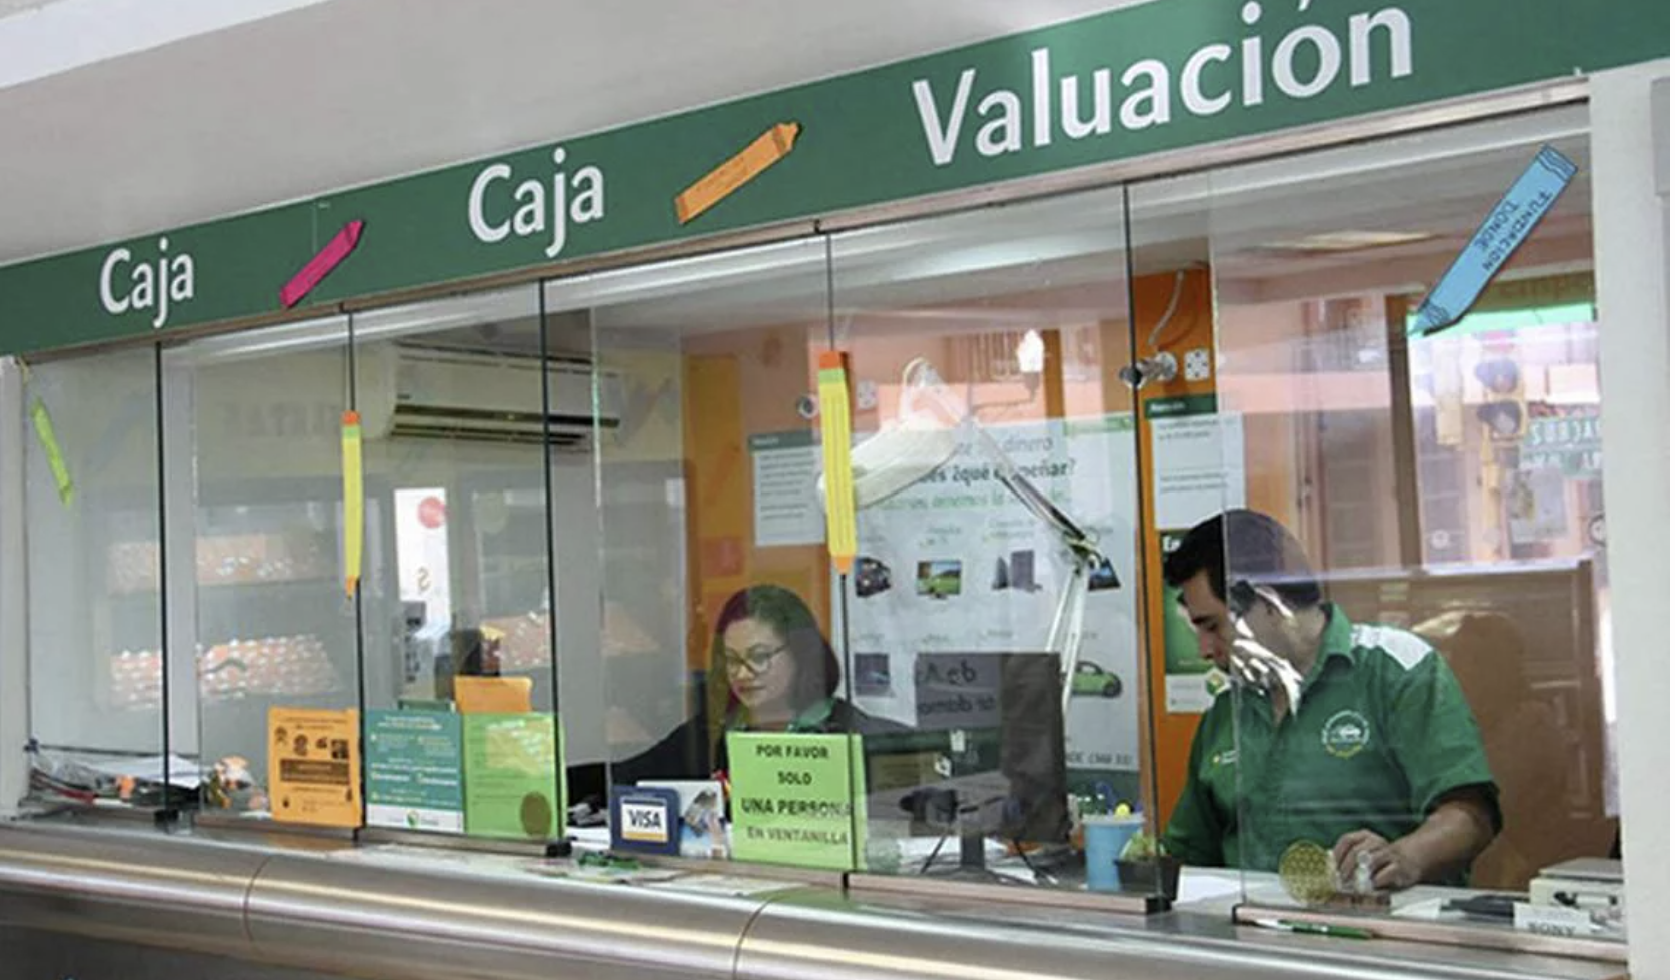
\includegraphics[width=0.95\textwidth]{Figuras/empenio9.png}
    \end{center}
    \end{figure}    
    \end{column}
\begin{column}{.45\textwidth}
\begin{figure}[H]
    \begin{center}
    \caption{Waiting for appraisal}
        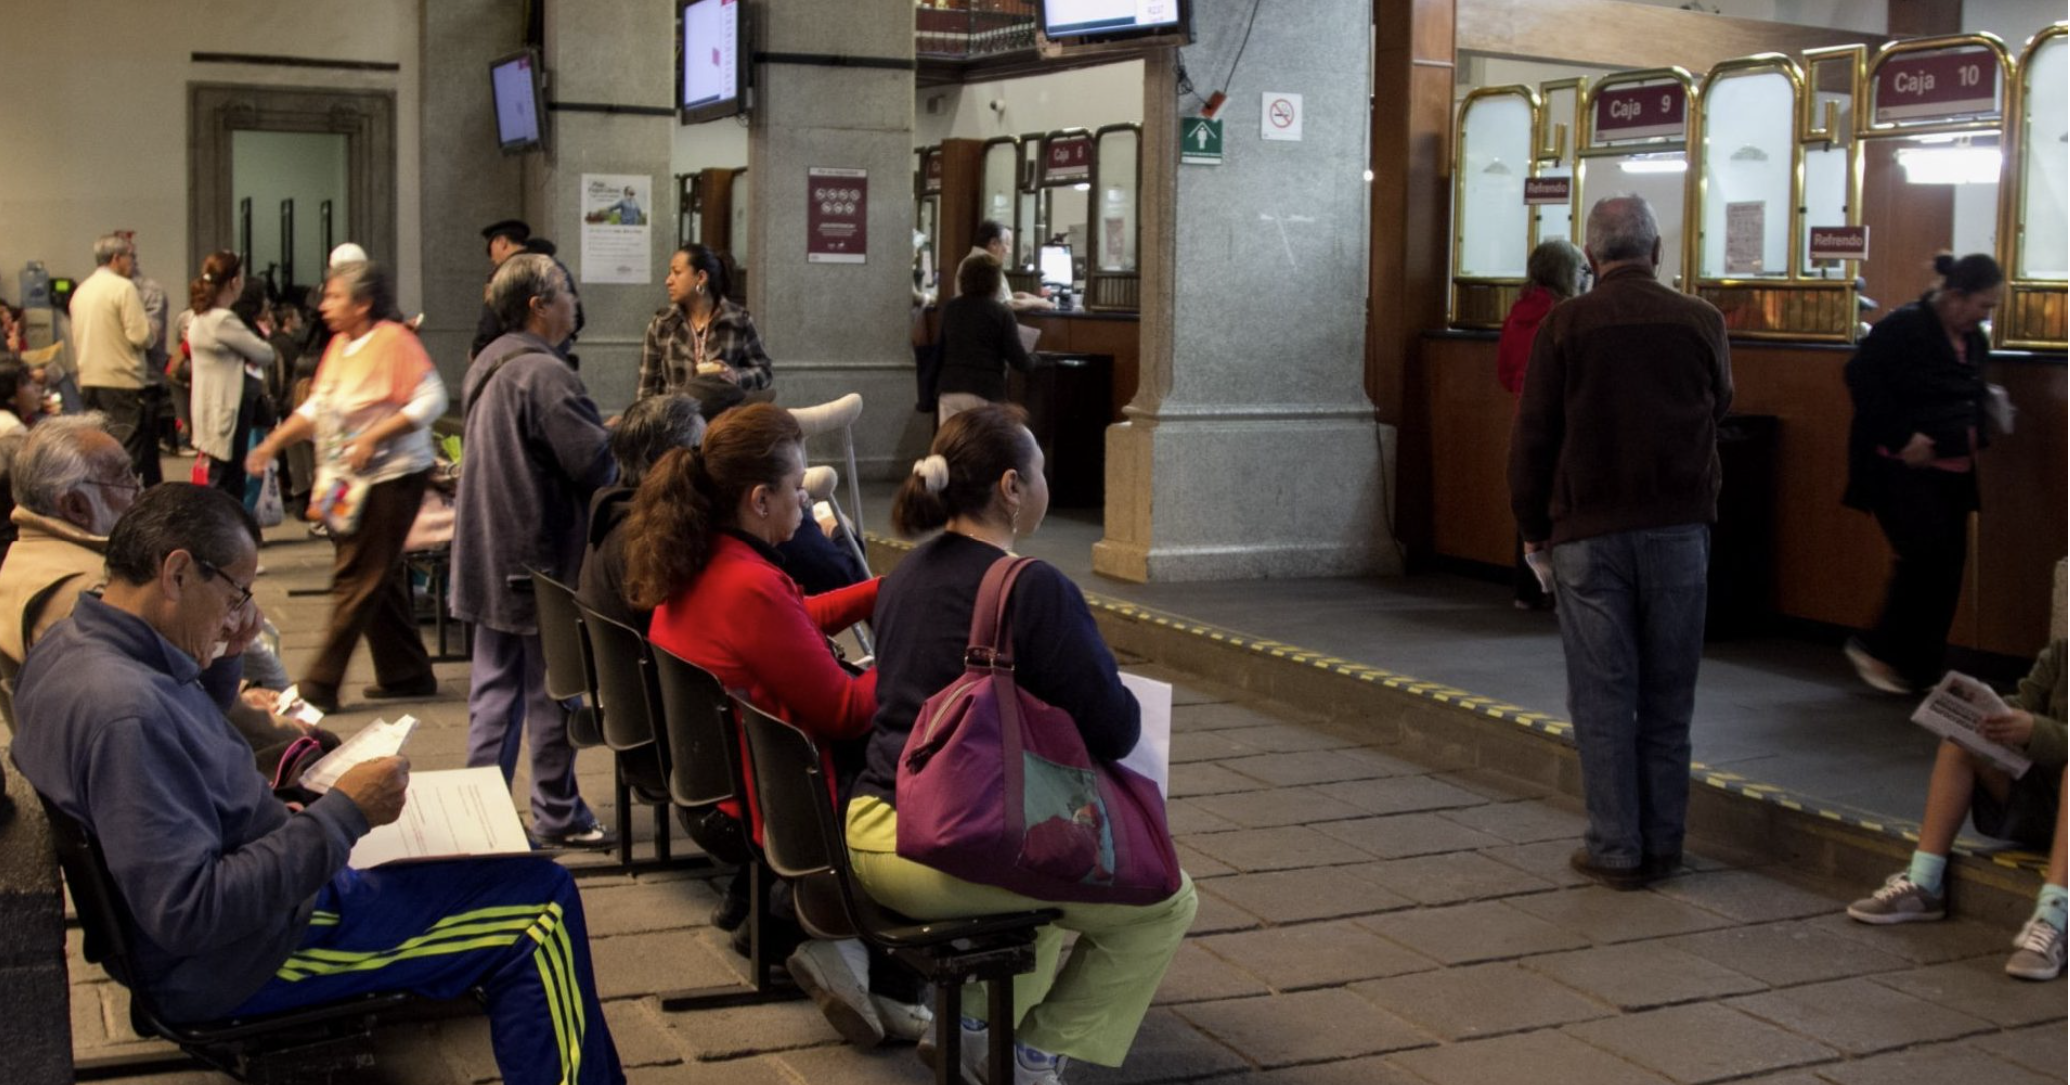
\includegraphics[width=0.95\textwidth]{Figuras/empenio11.png}
    \end{center}
    \end{figure}
\begin{figure}[H]
    \begin{center}
    \caption{Lost pawns which are for sale}
        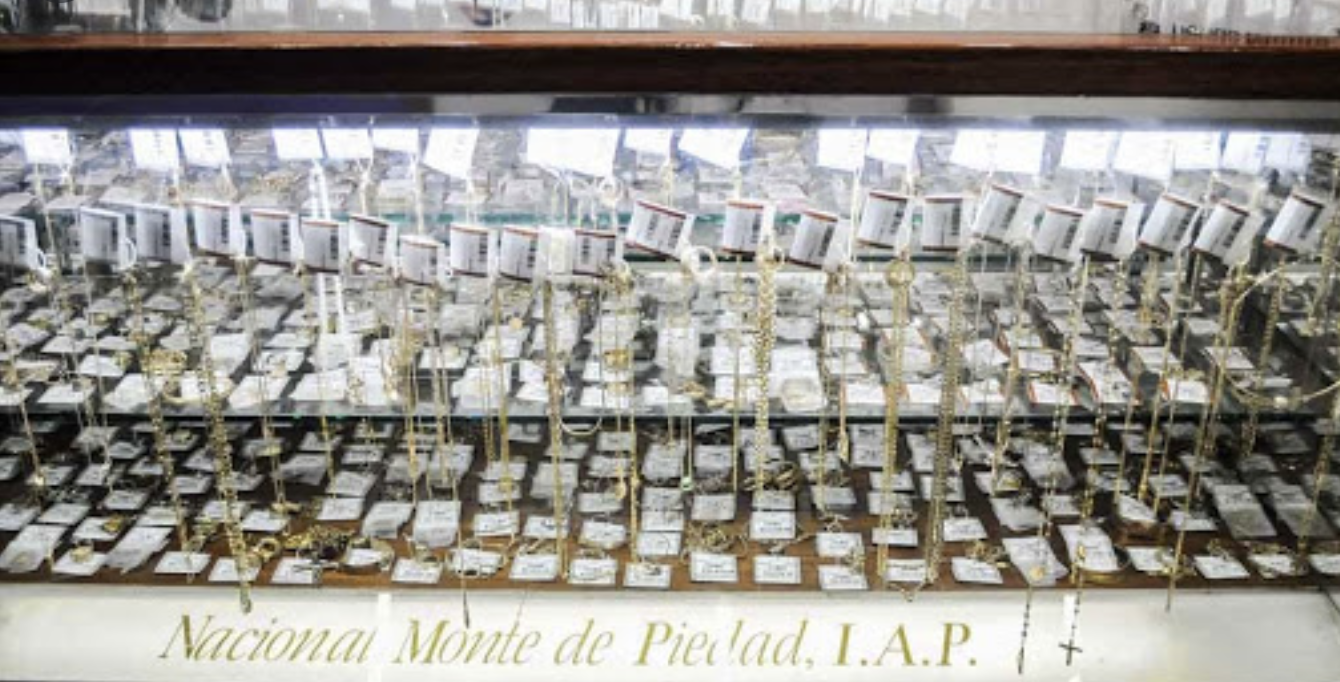
\includegraphics[width=0.95\textwidth]{Figuras/empenio3.png}
    \end{center}
    \end{figure}    
    \end{column}    
    \end{columns}
\end{frame}


\begin{frame}{Context}
\begin{itemize}
    \vfill \item Pawn loans involve borrowers leaving valuable liquid assets as collateral in exchange for an immediate cash loan
    \vfill \pause \item The loan is overcollateralized (loan is 70\% of appraised value) and collateral is liquid.
    \begin{itemize}
        \item The lender approves loans in a few minutes without income or credit history check $\rightarrow$ used for emergencies.
    \end{itemize}
  \vfill \pause \item Because the loan is overcollateralized and collateral is liquid, the lender may gain if the borrower defaults on the loan, especially if the borrower pays towards recovery on the way to default.
    \vfill \pause  \item Among those that lose their pawn (60\%), 48\% paid a positive amount towards its recovery and on average paid 42\% of loan.
    \vfill      \item This happens in spite (or because?) of 74\% of borrowers reporting a 100\% subjective probability recovery ex-ante. 
    %\vfill   \item 13\% of borrowers are classified as present biased using the simple standard question.
     \vfill \pause    \item In such an environment, one may ask if putting more structure/committment in payments may help borrowers recover their pawn.
     \vfill \pause    \item Not only that: Will the structure/commitment be demanded by all (or most) people who benefit?
        

\end{itemize}
\end{frame}





\section{Contribution}

\begin{frame}{Methodological Contribution}
\begin{itemize}
 %\vfill \item A context of particular interest to behavioral literature:  the demand for commitment in financial contracts (Laibson 1997, Bryan et al. 2010), and many more.
 
   \vfill   \item Key quantity in debate about paternalism:  impacts on those who wouldn't elect to take the program versus impacts on those that do.   \begin{itemize}
       \item Oreopoulos 2006: effect of mandatory high school laws.
       \item Fowlie et al. 2021: defaulting customers into variable electricity pricing.
   \end{itemize} 
   
   
   
   
   %How do treatment effects relate to selection?  
    
    %Broadly speaking there are two approaches: the structural approach and the reduced form approach.

    %The structural approach combines instruments with a generalized Roy model and uses behavioral and statistical restrictions to extrapolate the causal effects for different sub-populations
    
    
    %The structural approach allows both selection on unobservables and selection on gains at the cost of modeling these channels. In contrast, the reduced form approach assumes that there is no selection on gains after conditioning on a set of covariates 


    \vfill \item  Large literature TE heterogeneity: \begin{itemize}
        \item LATE-and-reweight:  Aronow \& Carnegie (2013); Angrist \& Fernandez Val (2013). \alert{Assume no selection on gains}
        \item Structurally model selection:  Walters (2018) \alert{Need their parametric models to be correct}.
        %TUT and ATE implied by LATE-and-re-weight differ sharply from his model-based estimates
        \item MTE: Heckman \& Vytlacil MTE; Cornelissen et. al. (2018). \alert{Need instrumental variable with rich support, and separability of observed and unobserved determinants of TE.}
        %\item Brinch et. al. (2017) - discrete $Z$ but under some additivity restrictions on the MTE curve
        %\item Mogstad, Santos \& Torgovitsky (2018) - No parametric form assumption on MTE curve but only partial identification.
    \end{itemize}

    \vfill \item Our ``Controlled Choice'' design point identifies a number of relevant TE with mild assumptions
    \begin{itemize}
        \item Because we have two forcing-arms and a choice arm, we can use one IV to get at ToT, and a second IV to get at TuT.
    \end{itemize}
    
    
   \vfill  \item Consider winners and losers from paternalism.     

%   \vfill \pause  \item Three-arm design:  Control, Choice (voluntary takeup=ITT), Forcing (universal=ATE).  We illustrate how to use standard exclusion restrictions to point identify:
%     \begin{itemize}
%         \item Treatment on the Treated (ToT) and 
%         \item Treatment on the Untreated (TUT), also
% 	\item Average Selection on Gains, Average Selection Bias, and Average Selection on Levels
%     \end{itemize} 
    
  


\end{itemize}
\end{frame}




\section{Outline}
\begin{frame}{Outline}
     \begin{itemize}
         \vfill\item \textbf{Experimental Design}
         \vfill\item Main results
         \vfill\item Paternalism
     \end{itemize}
\end{frame}







\section{Design}


\begin{frame}{Pawn contract}
    \begin{figure}[H]
    \label{ExplanatoryMaterial}
    \begin{center}
        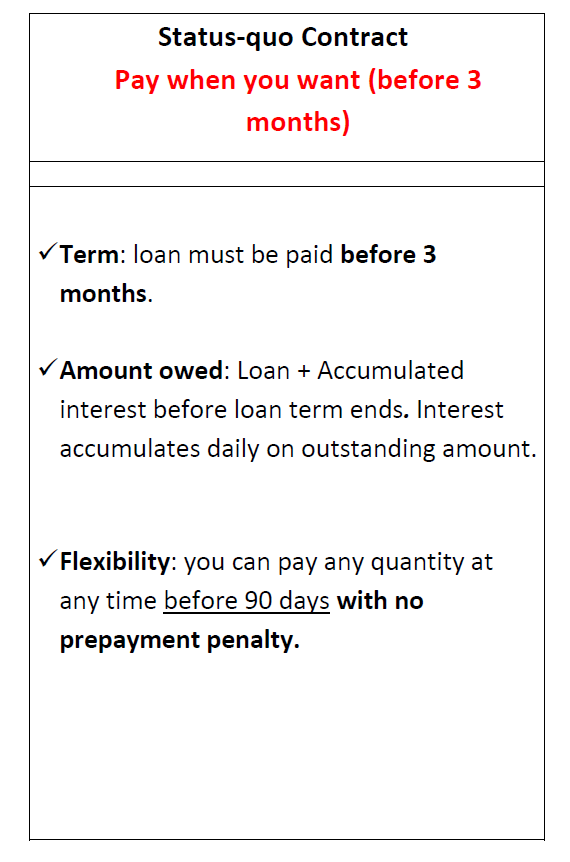
\includegraphics[width=0.45\textwidth]{Figuras/sq_contract.png}
    \end{center}
\end{figure}
\end{frame}




\begin{frame}{Structured payments contract}
   \begin{itemize}
       \vfill \item We designed a new contract that is identical to the status quo contract except that it enhances the regularity and salience of payments as a way to encourage repayment.
         \begin{figure}[H]
    \label{ExplanatoryMaterial}
    \begin{center}
        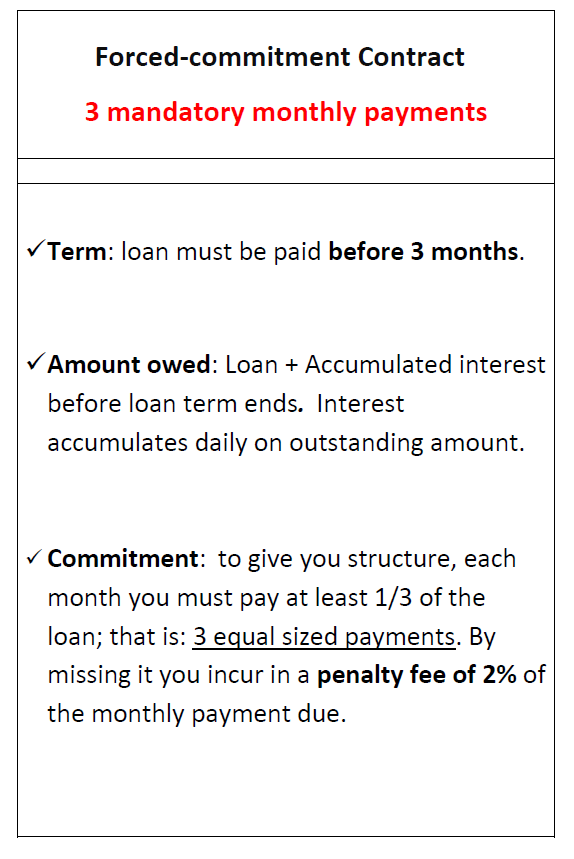
\includegraphics[width=0.40\textwidth]{Figuras/fc_contract.png}
    \end{center}
\end{figure}
       
   \end{itemize}
    
\end{frame}

% \begin{frame}{Structured payments contract}
%   \begin{itemize}
     
%       \vfill\item The purpose of the small fee was to mainly to make the structured schedule salient, not to be a large disincentive to be late. 
%       \begin{itemize}
%           \item Transportation cost to go to the branch to pay is on the same order of magnitude as the fee in average.
%       \end{itemize}
%       \vfill\item  The empirical literature provides some guidance that such a contract may decrease default and elicit demand.
%       \begin{itemize}
%           \item Field \& Pande (2008) find null effects of payment frequency on loan default for group lending (but samples are small and there is almost no default in the control). 
    
%         \item  Bauer et al. (2012) estimate a positive correlation between measured present bias and selecting into microfinance, which they interpret as demand for structured payments.
%       \end{itemize}
       
%   \end{itemize}
    
% \end{frame}

\begin{frame}{Data}
\label{data}
\begin{itemize}
    \item Administrative data: 1 month before and 8 months after the experiment ended
    \begin{itemize}
        \item Unique identifier for each client and each pawn.
        \item Value of the item, money loaned (70\%), date of pawning
        \item For all payments: date and amounts
        \item Fees incurred
        \item Whether the client lost the pawn, renewed the contract
    \end{itemize} 

    \vfill \item Survey data
    \begin{itemize}
        \item During experiment, we asked clients to complete a 5-minute survey before going to the teller window to appraise their piece and before treatment status was known to them.
        \item Demographics, proxies for income/wealth, education, present-biased preferences, experience pawning, if family or friends commonly asked for money, cost of going to branch, the subjective probability of recovering, the subjective value, etc.
    \end{itemize}
\end{itemize}    
\end{frame}


\begin{frame}{Main outcomes: financial cost and default}
\label{fc_outcome}
\begin{itemize}
    \item We are interested in measuring the financial cost of borrowing, which very saliently includes the cost of defaulting on the loan and losing the pawn.
    \item We will measure loan default using an indicator $\mathds{1}(\text{Default}_i)$, and the cost in pesos using the following definition that capture borrower outlays:
\end{itemize}

   \begin{equation*}
    \text{Financial Cost}_i =  \underbrace{\sum_t P^i_{it}}_{\text{Pay to Interest}} + \underbrace{\sum_t P^f_{it}}_{\text{Pay to Fees}}  + \mathds{1}(\text{Default}_i) \times \left[\text{Pawn Val}_i + \underbrace{\sum_t P^c_{it}}_{\text{Pay to Capital}} \right]
   \end{equation*}

\vspace{.2in}
\: \: \: \: APR: equivalent yearly interest generated by sum of payments:
   \begin{equation*}
    (\text{APR})_i =\left( 1 + \frac{\frac{\text{Financial Cost}_i}{\text{Appraised Value}_i}}{\text{loan term}_i}\right)^{\text{loan term}_i}-1 
\end{equation*}

   \vspace{.2in}
\begin{itemize}
    \item We \alert{will not talk about welfare}, only financial cost.
    \begin{itemize}
        \item Welfare would depend on reduced liquidity, anxiety from monthly payments, cost of going to branch, etc. We don't observe these.
    \end{itemize}
\end{itemize}
\end{frame}







\begin{frame}{Treatment arms}
\label{treatment_arms}
   \begin{itemize}
    \vfill \item Randomization at the branch-day level.  Analysis at the pawn level.
    \begin{itemize}
        \vfill \item Control arm (1770 obs)
       \vfill \item Forced Commitment arm (1954 obs)
       \vfill \item Choice Commitment arm (2580 obs)
    \end{itemize}
    \vfill \item The existence of a choice arm allows us not only to measure if there is demand for such a contract, but who demands it, not only in demographic terms, but in terms of potential treatment effects (which include unobservables).
   \vfill \item  This design is innovative and critical for our purposes, as it enables us to explore whether or not forcing people into a structured payment contract could be more beneficial than allowing choice for a significant fraction of them.
\end{itemize}
\end{frame}


% \begin{frame}{Description}
% \label{consort}
% \begin{figure}[H]
%      \caption{Experiment description}
%     \label{exp_description}
% \begin{center}
%         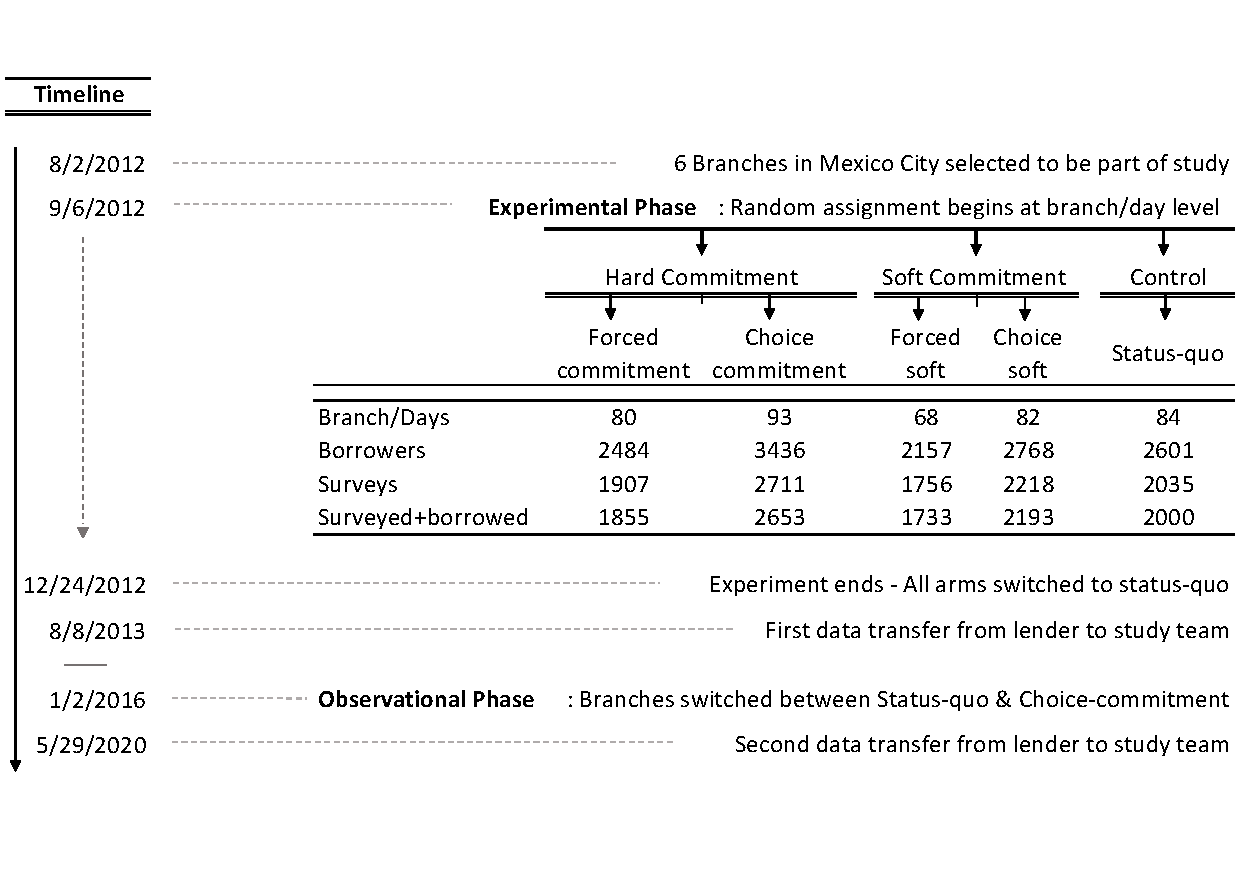
\includegraphics[width=0.80\textwidth]{Figuras/consort.pdf}
%   \end{center}
% \end{figure}
% \hyperlink{experimental_integrity}{\beamerbutton{Details}}

% \end{frame}




\begin{frame}{Experimental integrity}
\label{experimental_integrity}
    \begin{table}[H]
\caption{Attrition table}
\label{attrition_table}
\begin{center}
\small{% Table generated by Excel2LaTeX from sheet 'Attrition'
\begin{tabular}{lcccr}
\toprule
      & Control & Structure & Choice & \multicolumn{1}{c}{p-value} \\
\midrule
\midrule
Loan take-up & 0.967 & 0.955 & 0.961 & 0.82 \\
      & (0.01) & (0.01) & (0.01) &  \\
\midrule
Number of borrowers & 20.8  & 22.2  & 25.4  & 0.17 \\
      & (3.29) & (3.9) & (4.89) &  \\
\rowcolor[rgb]{ .949,  .949,  .949} \multicolumn{1}{r}{median} & 19    & 20    & 21    & 0.5 \\
\midrule
Number of pawns/borrower & 1.4   & 1.4   & 1.4   & 0.43 \\
      & (0.08) & (0.04) & (0.05) &  \\
\rowcolor[rgb]{ .949,  .949,  .949} \multicolumn{1}{r}{median} & 1.4   & 1.3   & 1.3   & 0.6 \\
\midrule
Number of pawns  & 31    & 31.3  & 37.2  & 0.24 \\
      & (5.8) & (5.6) & (7.9) &  \\
\rowcolor[rgb]{ .949,  .949,  .949} \multicolumn{1}{r}{median} & 27    & 28    & 30    & 0.46 \\
\midrule
Amt borrowed/borrower & 2266.8 & 2094  & 2115.2 & 0.18 \\
      & (101.8) & (83.7) & (99.9) &  \\
\rowcolor[rgb]{ .949,  .949,  .949} \multicolumn{1}{r}{median} & 2154.3 & 2041  & 2047.5 & 0.65 \\
\midrule
Total borrowed & 47877 & 47813 & 54780 & 0.4 \\
      & (8005) & (9436) & (12587) &  \\
\rowcolor[rgb]{ .949,  .949,  .949} \multicolumn{1}{r}{median} & 37520 & 39420 & 40850 & 0.73 \\
\midrule
Obs   & 85    & 81    & 94    &  \\
\bottomrule
\bottomrule
\end{tabular}%
}
\end{center}
\end{table}
\end{frame}



\begin{frame}{Balance and Summary statistics}
    \begin{table}[H]
%\caption{Summary statistics and Balance}
\label{SS}
\begin{center}
\resizebox{.65\textwidth}{!}{
\scriptsize{% Table generated by Excel2LaTeX from sheet 'SS'
\begin{tabular}{lcccccccc}
\toprule
      &       &       & \multicolumn{5}{c}{Treatment arms}    &  \\
\midrule
      &       &       &       & \multicolumn{2}{c}{No Choice } & \multicolumn{2}{c}{Choice} &  \\
\midrule
\midrule
      & Overall & Pre-experiment & Control & Fee   & Promise & Fee   & Promise & p-value \\
\midrule
      & \multicolumn{8}{c}{Panel A : Administrative Data} \\
\midrule
\midrule
Loan amount  & 2197  & 2239  & 2301  & 2147  & 2133  & 2181  & 2089  & 0.32 \\
      & (25)  & (39)  & (79)  & (72)  & (74)  & (65)  & (65)  &  \\
Monday & 0.18  & 0.16  & 0.18  & 0.16  & 0.17  & 0.19  & 0.21  & 0.96 \\
      & (0.02) & (0.03) & (0.05) & (0.05) & (0.06) & (0.06) & (0.05) &  \\
Number of branch-day pawns & 34    & 36    & 31    & 31    & 32    & 37    & 34    & 0.38 \\
      & (0.82) & (1.25) & (2.2) & (2.35) & (2.38) & (2.65) & (1.76) &  \\
\midrule
Number of branch-days & -     &       & 84    & 80    & 68    & 93    & 82    &  \\
Obs   & 21808 & 8366  & 2601  & 2484  & 2156  & 3435  & 2766  &  \\
\midrule
      & \multicolumn{8}{c}{Panel B : Survey Data (conditional on pawning)} \\
\midrule
\midrule
Woman & 0.73  &       & 0.76  & 0.72  & 0.73  & 0.72  & 0.74  & 0.41 \\
      & (0.01) &       & (0.02) & (0.02) & (0.02) & (0.02) & (0.01) &  \\
Age   & 43.31 &       & 43.16 & 43.17 & 42.96 & 43.96 & 43.06 & 0.79 \\
      & (0.28) &       & (0.57) & (0.79) & (0.65) & (0.61) & (0.52) &  \\
Subjective value & 3068  &       & 3151  & 2978  & 2985  & 3114  & 3079  & 0.41 \\
      & (39)  &       & (69)  & (91)  & (76)  & (85)  & (100) &  \\
Has pawn before & 0.9   &       & 0.89  & 0.9   & 0.89  & 0.91  & 0.89  & 0.68 \\
      & (0)   &       & (0.01) & (0.01) & (0.01) & (0.01) & (0.01) &  \\
Subj. pr. of recovery & 93.14 &       & 92.74 & 92.16 & 93.6  & 93.67 & 93.3  & 0.46 \\
      & (0)   &       & (0.55) & (0.86) & (0.6) & (0.47) & (0.6) &  \\
+High-school & 0.66  &       & 0.66  & 0.67  & 0.65  & 0.67  & 0.64  & 0.74 \\
      & (0.01) &       & (0.02) & (0.02) & (0.02) & (0.02) & (0.02) &  \\
Survey response rate & 0.78  &       & 0.77  & 0.75  & 0.8   & 0.77  & 0.79  & 0.5 \\
      & (0.01) &       & (0.02) & (0.03) & (0.02) & (0.02) & (0.02) &  \\
\midrule
Obs   & 10431 &       & 2000  & 1855  & 1732  & 2652  & 2192  &  \\
\midrule
\midrule
      & \multicolumn{8}{c}{Panel C : Survey Data (unconditional)} \\
\midrule
\midrule
Woman & 0.74  & 0.75  & 0.76  & 0.72  & 0.73  & 0.72  & 0.74  & 0.32 \\
      & (0.01) & (0.01) & (0.02) & (0.02) & (0.02) & (0.02) & (0.01) &  \\
Age   & 43.24 & 43.06 & 43.2  & 43.21 & 43.01 & 44.07 & 43.07 & 0.79 \\
      & (0.21) & (0.32) & (0.56) & (0.77) & (0.66) & (0.61) & (0.51) &  \\
Subjective value & 3112  & 3192  & 3145  & 2985  & 3010  & 3111  & 3082  & 0.41 \\
      & (36)  & (75)  & (68)  & (88)  & (76)  & (84)  & (99)  &  \\
Has pawn before & 0.89  & 0.88  & 0.89  & 0.9   & 0.89  & 0.91  & 0.89  & 0.56 \\
      & (0.01) & (0.01) & (0.01) & (0.01) & (0.01) & (0.01) & (0.01) &  \\
Subj. pr. of recovery & 92.64 & 91.84 & 92.73 & 92.19 & 93.66 & 93.71 & 93.34 & 0 \\
      & (0.2) & (0.31) & (0.54) & (0.84) & (0.59) & (0.46) & (0.59) &  \\
+High-school & 0.63  & 0.6   & 0.66  & 0.67  & 0.65  & 0.66  & 0.64  & 0.01 \\
      & (0.01) & (0.01) & (0.02) & (0.02) & (0.02) & (0.02) & (0.02) &  \\
\% ended up pawning &       &       & 0.98  & 0.97  & 0.99  & 0.98  & 0.99  & 0.25 \\
\midrule
Obs   & 17546 & 6919  & 2035  & 1907  & 1757  & 2710  & 2218  &  \\
\bottomrule
\bottomrule
\end{tabular}%
}
}
\end{center}
%\textit{Do file: } \texttt{ss\_att.do}
\end{table}
% \hyperlink{data}{\beamerbutton{Back}}
\end{frame}




\begin{frame}
\textbf{Predictors of take-up : $\Pr(Take-up)$}

\begin{figure}[H]
    \begin{center}
        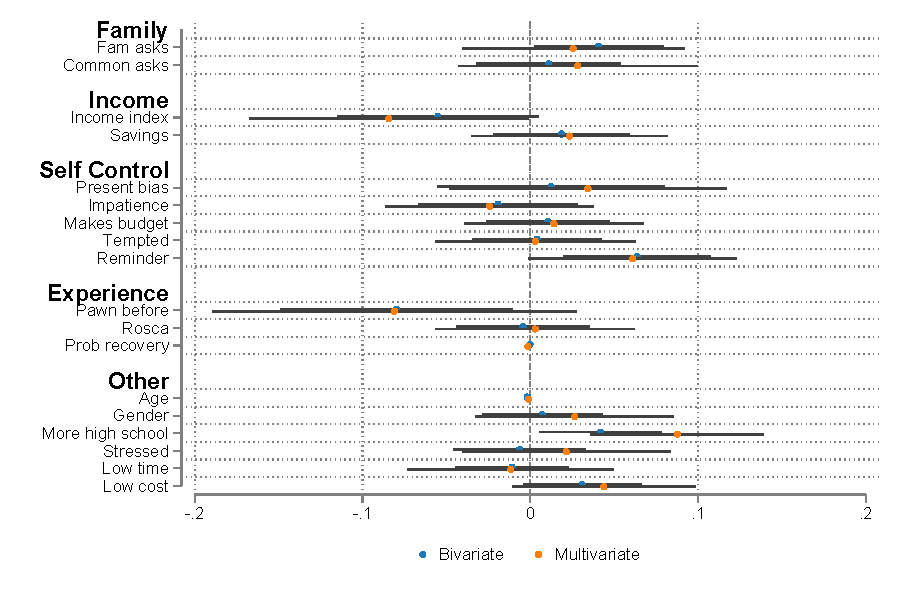
\includegraphics[width=0.9\textwidth]{Figuras/determinants_takeup_reg.pdf}
    \end{center}
    \end{figure}
\end{frame}





\begin{frame}{Outline}
     \begin{itemize}
         \vfill\item Experimental Design
         \vfill\item \textbf{Main results}
         \vfill\item Paternalism 
     \end{itemize}
\end{frame}





\section{Main Results}
\begin{frame}{Main results: ITT}
\label{main_results}


\begin{itemize}
    \item Financial cost reduced by \$379 pesos (20\% of mean). That is: charging fee + structure \textit{decreased} cost.
    \item Default decreases by 6.5pp (15\% of mean).
    \item APR decreases by 34 points, from mean of 184.
\end{itemize}
\vspace{.3in}
\begin{table}[H]
\begin{center}
\resizebox{0.95\textwidth}{!}{
\small{% Table generated by Excel2LaTeX from sheet 'decomposition_main_te_pres1'
\begin{tabular}{lcccccc}
\toprule
      &       & \multicolumn{5}{c}{Components of FC} \\
\cmidrule{3-7}      & FC    & \textcolor[rgb]{ .749,  .749,  .749}{Int. pymnt} & \textcolor[rgb]{ .749,  .749,  .749}{Fee pymnt} & \textcolor[rgb]{ .749,  .749,  .749}{Princ. pymnt} & \textcolor[rgb]{ .749,  .749,  .749}{Lost pawn val} & Default \\
\midrule
      & (1)   & \textcolor[rgb]{ .749,  .749,  .749}{(2)} & \textcolor[rgb]{ .749,  .749,  .749}{(3)} & \textcolor[rgb]{ .749,  .749,  .749}{(4)} & \textcolor[rgb]{ .749,  .749,  .749}{(5)} & (6) \\
\midrule
\midrule
Forced cmit & \boxit{0.5in} -379.7*** & \textcolor[rgb]{ .749,  .749,  .749}{-157.3***} & \textcolor[rgb]{ .749,  .749,  .749}{32.1***} & \textcolor[rgb]{ .749,  .749,  .749}{-0.57} & \textcolor[rgb]{ .749,  .749,  .749}{-254.5**} & \boxit{0.5in} -0.065*** \\
      & (111.4) & \textcolor[rgb]{ .749,  .749,  .749}{(34.9)} & \textcolor[rgb]{ .749,  .749,  .749}{(1.43)} & \textcolor[rgb]{ .749,  .749,  .749}{(3.03)} & \textcolor[rgb]{ .749,  .749,  .749}{(104.8)} & (0.023) \\
Choice cmit & -84.9 & \textcolor[rgb]{ .749,  .749,  .749}{-24.9} & \textcolor[rgb]{ .749,  .749,  .749}{1.34**} & \textcolor[rgb]{ .749,  .749,  .749}{-3.98} & \textcolor[rgb]{ .749,  .749,  .749}{-61.4} & -0.025 \\
      & (114.6) & \textcolor[rgb]{ .749,  .749,  .749}{(38.4)} & \textcolor[rgb]{ .749,  .749,  .749}{(0.54)} & \textcolor[rgb]{ .749,  .749,  .749}{(2.47)} & \textcolor[rgb]{ .749,  .749,  .749}{(109.2)} & (0.021) \\
      &       & \textcolor[rgb]{ .749,  .749,  .749}{} & \textcolor[rgb]{ .749,  .749,  .749}{} & \textcolor[rgb]{ .749,  .749,  .749}{} & \textcolor[rgb]{ .749,  .749,  .749}{} &  \\
\midrule
Observations & 6304  & \textcolor[rgb]{ .749,  .749,  .749}{6304} & \textcolor[rgb]{ .749,  .749,  .749}{6304} & \textcolor[rgb]{ .749,  .749,  .749}{6304} & \textcolor[rgb]{ .749,  .749,  .749}{6304} & 6304 \\
R-squared & 0.007 & \textcolor[rgb]{ .749,  .749,  .749}{0.022} & \textcolor[rgb]{ .749,  .749,  .749}{0.151} & \textcolor[rgb]{ .749,  .749,  .749}{0.003} & \textcolor[rgb]{ .749,  .749,  .749}{0.007} & 0.013 \\
Control Mean & 1851.0 & \textcolor[rgb]{ .749,  .749,  .749}{545.9} & \textcolor[rgb]{ .749,  .749,  .749}{0} & \textcolor[rgb]{ .749,  .749,  .749}{5.82} & \textcolor[rgb]{ .749,  .749,  .749}{1305.1} & 0.44 \\
\bottomrule
\bottomrule
\end{tabular}%
}
}
\end{center}
\end{table}

   \vfill 
  \hyperlink{several_def_cost}{\beamerbutton{More}}

\end{frame}




\begin{frame}{Intermediate outcomes: forced-commitment}
\label{intermediate_outcomes}
 \begin{itemize}
     \item \vfill \textbf{Speed of payment:} The first payment of the forced commitment contract  occurs 13 days earlier, increasing the fraction who recover on the first visit by 7.9 pp. Conditional on recovering, they recover 28 days faster.
     
    \item \vfill \textbf{Separating those who will not pay:} Commitment contract decreases fraction of borrowers making a payment and \textit{not} recovering by 7pp.
    \begin{itemize}
        \item Actually, among those that default, those in the forced commitment arm are 14pp less likely to have paid towards recovery. They also visit the branch less: as if the commitment contract makes them realize they will end up losing pawn anyway, and stop paying early on.
    \end{itemize}
    \end{itemize}

   \vfill
   
   \hyperlink{mechanism_appendix}{\beamerbutton{Details}}
\end{frame}


\section{Paternalism}
\begin{frame}{Choice and Heterogeneous Treatment Effects}
\label{choice_hte}
    \begin{itemize}
    \vfill \item  So, forcing commitment decreases APR dramatically. 
    
    \vfill \item \textbf{Low demand:} In spite of this, given the opportunity, only 11\% of borrowers chose commitment.   
    \begin{itemize}
       \pause \item If the effect of commitment were homogeneous, this would be enough to conclude that the 89\% who did not choose it would have been financially better off if they had.
       \item However, we test and reject the null hypothesis of homogeneous treatment effects (Chernozhuvok et. al. 2018).
    \end{itemize}
    
    \vfill \item The borrowers who did not choose commitment could simply be those who don’t need it?
    \pause \vfill \ item The distribution of TE (i.e. $Y_{1i}-Y_{0i}$) is not identified, as one person is only observed in one treatment. However, it can be bounded using the two marginal dist $F_1$ and $F_0$. \hyperlink{fan_park_bounds}{\beamerbutton{Fan \& Park bounds}}
    \vfill \item \textbf{Many with benefits did not demand:} We find that at least 30\% of individual borrowers benefit from commitment $\implies$ many did not demand even though TE is positive for them.
    \vfill \item Given our 3-armed experiment (+ imposing a mean exclusion restriction) allow us to estimate average TuT$>0$. %Furthermore, imposing the restriction for each cell of covariates and using Causal Forests gets us $F_{TUT}^{-1}(0.72)>0$.
    \end{itemize}
\end{frame}

 
\begin{frame}{Identification afforded by experiment}

\vspace{.2in}
Notation: 
\begin{itemize}
    \item Potential outcomes $(Y_0,Y_1,C)$
    \item Assignment: $Z \in \{0,1,2\}$, i.e. \{SQ,Com,Choice\}.  
    \item Treatment: $D \in \{0,1\} $, i.e. \{SQ,Com\}.
\end{itemize}

\vspace{.2in}
Assumptions:

\begin{itemize}
    \item $Z \independent (Y_0,Y_1,C)$, achieved by randomization
    \item $D = \mathbbm{1}(Z_i \neq 2) Z + \mathbbm{1}(Z_i=2) C$, i.e. \alert{being assigned to a contract has same effect as choosing it} (e.g. used in compulsory school attendance and returns to schooling lit).
\end{itemize}

\vspace{.2in}
Therefore:
\begin{itemize}
    \item  $Y_i = \mathbbm{1}(Z_i =0) Y_{i0} + \mathbbm{1}(Z_i = 1)  Y_{i1}  + \mathbbm{1}(Z_i = 2) \left[(1 - C_i) Y_{i0} + C_i Y_{i1} \right].$
\end{itemize}

\vspace{.2in}
Prop:
\begin{itemize}
    \item ToT := $\mathbbm{E}(Y_{i1} - Y_{i0} | C_i = 1)$ is point-identified, and equals $\frac{\mathbbm{E}(Y_i|Z_i=2) - \mathbbm{E}(Y_i|Z_i =0)}{\mathbbm{E}(D_i|Z_i=2)} $
     \item TuT := $\mathbbm{E}(Y_{i1} - Y_{i0} | C_i = 0)$ is point-identified, and equals $\frac{\mathbbm{E}(Y_i|Z_i=1) - \mathbbm{E}(Y_i|Z_i =2)}{1-\mathbbm{E}(D_i|Z_i=2)} $
     \item Also identified: $ASG:=ToT-TuT$, $ASB:= \E[Y_0 | C=1]-\E[Y_0 | C=0]$, and $ASL:= \E[Y_1 | C=1]-\E[Y_1 | C=0]$. 
\end{itemize}
\end{frame}





\begin{frame}{The ``Controlled Choice'' Design}
\label{cc_design}
\begin{itemize}
    \item Recall that under one-sided non-compliance (no always-takers), LATE=ToT.
\end{itemize}
\vspace{.2in}
\begin{figure}[H]
    \begin{center}
        \centering
        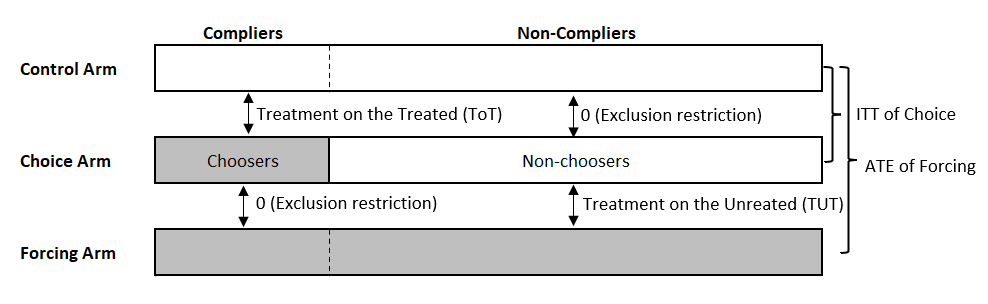
\includegraphics[width=1.0\textwidth]{Figuras/tot_tut_intuition.png}
    \end{center}
\end{figure}   
 \vfill
\hyperlink{identification_randomized_choice}{\beamerbutton{Identification}}
\end{frame}




\begin{frame}{On avg. those that do not choose would benefit: TuT $>$ 0}
\begin{itemize}
    \vfill \item Commitment increases average financial benefit even for the subset of borrowers who \alert{don't choose to commit voluntarily}.
    \vfill \item Coefficient ToT>TuT, but cannot reject equality due to large s.e. in ToT.
    \vfill \item Results hold when imputing transport cost and lost wages per visit, and charge interest in amount paid (as a proxy for liquidity lost).
\end{itemize}
\vspace{.2in}
\begin{table}[H]
%those who are most likely to benefit from it and those whose outcomes are most adverse under the status quo.
\label{tot_tut}
\begin{center}
\small{% Table generated by Excel2LaTeX from sheet 'tot_tut_pres1'
\begin{tabular}{lccc}
\toprule
      & FC benefit & \% (1-Default) & APR \\
\midrule
      & (1)   & (2)   & (3) \\
\midrule
\midrule
ToT $:= \E[Y_1 - Y_0 | C=1]$ & 668.3 & 38.7* & 132.7* \\
      & (1085.4) & (21.5) & (67.8) \\
TuT $:= \E[Y_1 - Y_0 | C=0]$ & 356.1*** & 3.98* & 24.0*** \\
      & (107.8) & (2.40) & (8.20) \\
\midrule
ASG := ToT-TuT & 312.2 & 34.7  & 108.7 \\
      & (1132.4) & (22.5) & (70.9) \\
ASB $:= \E[Y_0 | C=1]-\E[Y_0 | C=0]$ & -77.9 & -40.6* & -122.3* \\
      & (1127.5) & (22.2) & (70.5) \\
ASL $:= \E[Y_1 | C=1]-\E[Y_1 | C=0]$ & 234.3 & -5.90 & -13.6 \\
      & (154.4) & (4.29) & (15.9) \\
      &       &       &  \\
\midrule
Observations & 6304  & 6304  & 6304 \\
H_0 : ToT-TuT=0 & 0.78  & 0.12  & 0.13 \\
H_0 : ToT-TuT$\geq$ 0 & 0.39  & 0.062 & 0.063 \\
\bottomrule
\bottomrule
\end{tabular}%
}
\end{center}
\end{table}
\end{frame}

% Despite substantial treatment effect heterogeneity, most borrowers would experience higher financial benefits under a commitment contract : $F_{\operatorname{TUT}}^{-1}(0.72)>0$






\begin{frame}{Fraction that forgo benefit}


    \label{choose_wrong}
    
        \begin{figure}{\textwidth}
        \caption{Mistakes in choice arm}
        \centering
        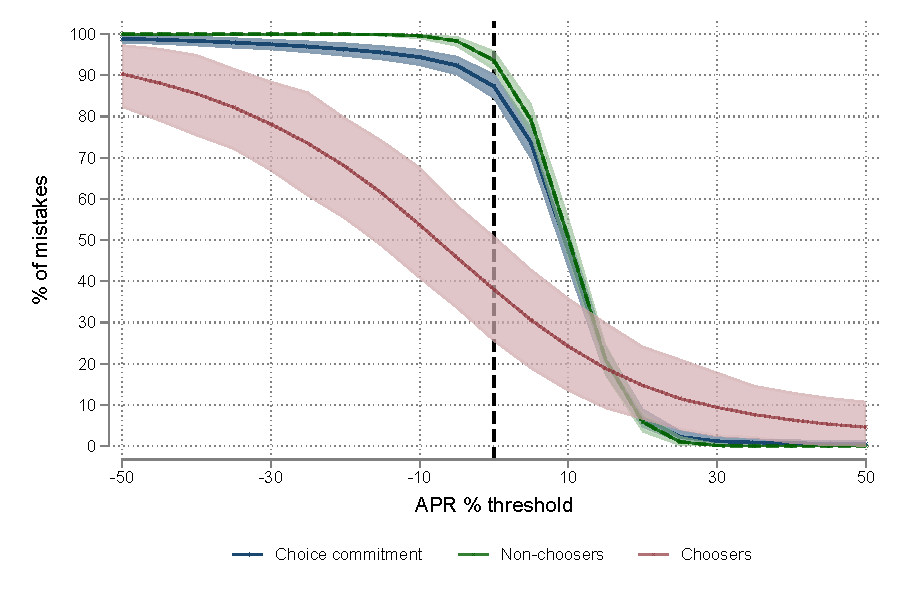
\includegraphics[width=0.65\textwidth]{Figuras/line_cw_apr_tot_tut.pdf}
        \end{figure}

\begin{itemize}
    \item   Use Random Forest to estimate ToT, TUT conditional on covariates.
    \item $>$ 70\% of non-choosers would have seen some benefit from assignment to commitment.
    \item  $<$ 20\% of choosers made a mistake.
\end{itemize}        


\end{frame}







\begin{frame}{Effects on clients coming back}

\begin{itemize}
    \item Client forced into commitment is 20\% more likely to come back again and pawn.
    \item Not mechanically from having recovered the pawned, since also pawn other pieces.
    \item Not within the life of the loan, but after. So unlikely that is a liquidity story.
    \item Conditional on recovery (endogenous), ``effect'' twice as big.
\end{itemize}

\vspace{.2in}
\begin{table}[H]
\begin{center}
\footnotesize{% Table generated by Excel2LaTeX from sheet 'repeat_loans'
\begin{tabular}{lcccccccc}
\toprule
      & \multicolumn{6}{c}{Ever pawns again (ITT)}    &       &  \\
\cmidrule{2-7}      &       & Cond. on rec & Cond. on default & Different collateral & After 90 days & Within 90 days &       & Days from 1st loan  \\
\midrule
\midrule
      & (1)   & (2)   & (3)   & (4)   & (5)   & (6)   &       & (7) \\
\midrule
\midrule
Forced commitment & 0.067* & 0.10** & -0.0046 & 0.036 & 0.037*** & 0.032 &       & 7.72** \\
      & (0.035) & (0.047) & (0.035) & (0.030) & (0.013) & (0.027) &       & (3.07) \\
Choice commitment & 0.040 & 0.051 & 0.026 & 0.027 & 0.0098 & 0.030 &       & 1.72 \\
      & (0.031) & (0.042) & (0.034) & (0.027) & (0.0087) & (0.026) &       & (2.59) \\
      &       &       &       &       &       &       &       &  \\
\midrule
Observations & 4441  & 2168  & 2273  & 4441  & 4441  & 4441  &       & 1577 \\
R-squared & 0.003 & 0.007 & 0.001 & 0.001 & 0.006 & 0.001 &       & 0.011 \\
Control Mean & 0.32  & 0.36  & 0.29  & 0.28  & 0.020 & 0.30  &       & 32.9 \\
\bottomrule
\bottomrule
\end{tabular}%
}
\end{center}
\end{table}    
\end{frame}



\begin{frame}{Learning}
    \label{learning_table}
    \begin{itemize}
    \item  Do people learn from Forced exposure to the program that they benefit from it?  
    \vspace{.1in}
    \item  Small sample (small power): focus on those that, after being either forced to commitment contract or to status quo, come back within a few months and are subject to choice arm.
    \vspace{.1in}
    \item  \textbf{No learning?} We don't find that being forced to the commitment contract makes them more likely to voluntarily chose commitment later.
    %\vfill \item Are people learning? \hyperlink{learning_table}{\beamerbutton{Table}}
 \end{itemize}  
 \vspace{.2in}
\begin{table}[H]
\begin{center}
\small{% Table generated by Excel2LaTeX from sheet 'learning_exp_pres'
\begin{tabular}{lc}
\toprule
      & Choose commitment \\
\cmidrule{2-2}$t-1$ & (1) \\
\midrule
\midrule
Forced commitment (ATE) & -0.0010 \\
      & (0.044) \\
Choice commitment (ITT) & 0.042 \\
      & (0.055) \\
      &  \\
\midrule
Observations & 240 \\
R-sq  & 0.005 \\
DepVarMean & 0.087 \\
\bottomrule
\bottomrule
\end{tabular}%
}
\end{center}
\end{table}
 %\hyperlink{learning}{\beamerbutton{Back}}
\end{frame}



\begin{frame}{If commitment works, why don't people choose it?}
    \begin{itemize}
        \onslide<1>{\item Discounting}
        \onslide<2-3>{\item Present-Bias}
    \end{itemize}
\vfill
\only<1>{  
 \begin{itemize}
 \item Can impatience explain why not take up a contract that decreases overall cost?
     \end{itemize}
\begin{figure}[H]
        \caption{Financial cost for different discount rates}
    \label{fc_discount_rates}
    \begin{center}
        \centering
        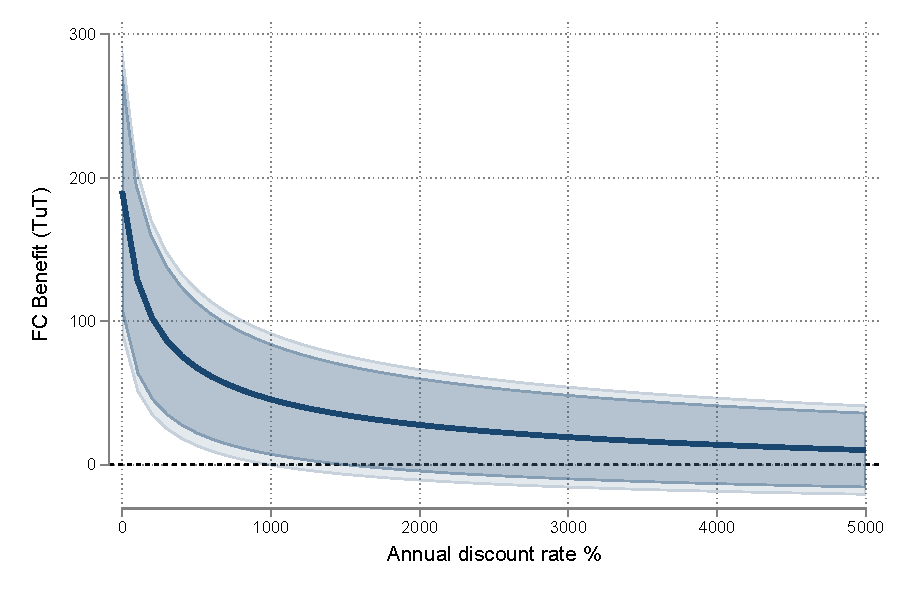
\includegraphics[width=0.50\textwidth]{Figuras/discount_effect_tut.pdf}
    \end{center}
\end{figure}   
    \begin{itemize}
    \item   Commitment contract imposes up-front costs for later benefits (collateral recovery).  
   
    \item  Requires an interest rate > 4,000\% to make NPV TuT insignificant. 
    \end{itemize}
}

\only<2>{  
  
    \begin{itemize}
    \item   Standard behavioral angle:  compliers are sophisticated time-inconsistent, non-compliers are a mix of naifs and the time consistent (who don't need commitment).  
    \end{itemize}
\begin{figure}[H]
    \begin{center}
        \centering
        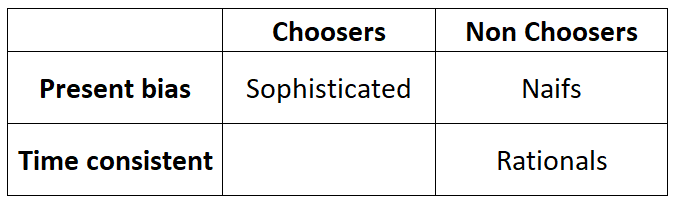
\includegraphics[width=0.65\textwidth]{Figuras/hyperbolicity_strata.png}
    \end{center}
\end{figure}   
    \begin{itemize}
    \item We have a survey measure of time inconsistency taken at baseline.
    \item  Effect of forcing commitment should be entirely among the time-inconsistent.  Is this true?  No, but PB measure may not be good.
    \end{itemize}
}

\only<3>{  
  
    \begin{itemize}
    \item   We estimate the TuT conditional on $X_i=1 or X_i=1$ (say $X_i= PB_i$ or $=Confidence_i$) and see which subpouplations have larger TuT.

\vspace{.3in}
    \begin{align*}
        1=& \frac{\mathbb{E}[Y_{1i}-Y_{0i} | D_i=0, X_i=1]}{TuT}\Pr(X_i=1 | D_i=0) \\
        \quad &+ \frac{\mathbb{E}[Y_{1i}-Y_{0i}| D_i=0, X_i=0]}{TuT}\Pr(X_i=0 | D_i=0)
    \end{align*}
    
%and we will say that the variable $B_i$ explains the ToT whenever one of the terms (ratio weighted by the probability) is statistically significant from zero, (close to one), and the other term is statistically zero.
    \end{itemize}
}
\end{frame}


\begin{frame}{Possible Behavioral explanations : TuT \& ToT by groups}

\begin{itemize}
    \item The TuT effect is concentrated on those that say they have 100\% of recovery. This is what we would expect if the Sure-confident don't demand because they think they don't need it (but are wrong).
    \item Also on those with no PB (as measured by us).
\end{itemize}
\begin{columns}
\begin{column}{.45\textwidth}
    \begin{figure}[H]
    \caption{TuT}
        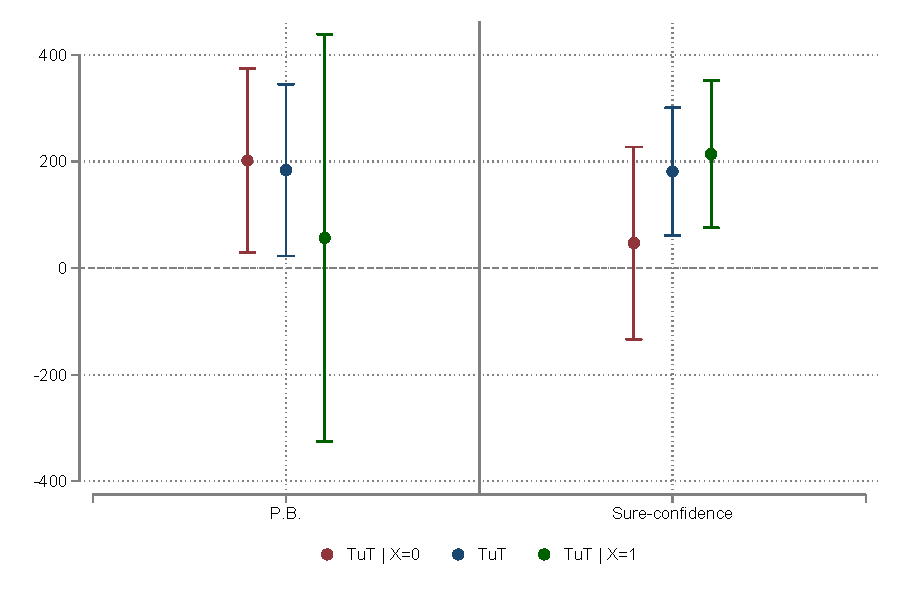
\includegraphics[width=1.1\textwidth]{Figuras/tut_beh_partition.pdf}
\end{figure}
\end{column}

\begin{column}{.45\textwidth}
    \begin{figure}[H]
    \caption{ToT}
        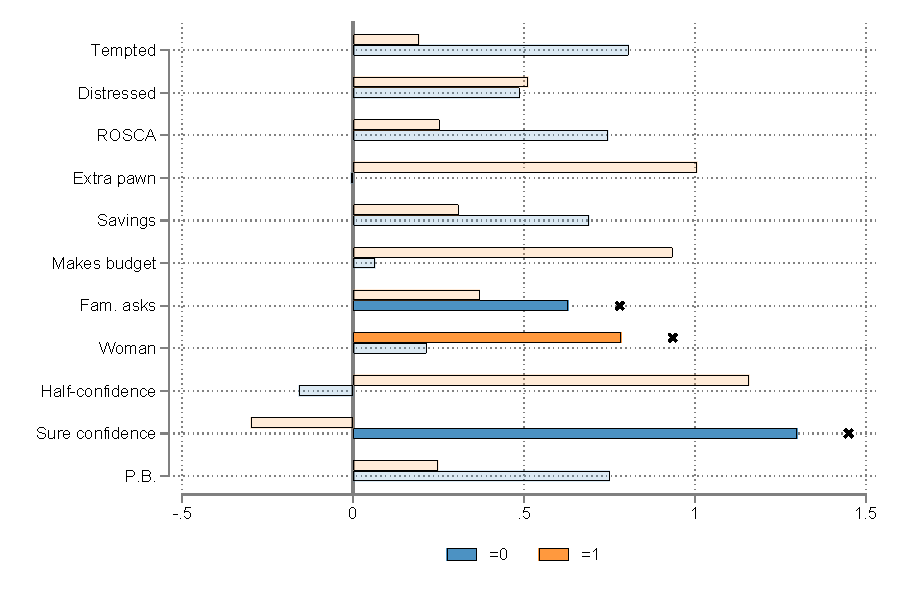
\includegraphics[width=1.1\textwidth]{Figuras/tot_beh_partition.pdf}
\end{figure}
\end{column}
\end{columns}
\end{frame}













\section{Conclusion}
\begin{frame}{Conclusion}
    \begin{itemize}
     \vfill \item Laibson has spoken of `veiled paternalism' in contexts where principals desire reliability; here we have a case of `veiled non-paternalism' where features encouraging default might be embedded.
     \vfill \item Novel design to study essential heterogeneity: ``Controlled Choice''
        %\begin{itemize}
         %   \item Combine ``Controlled Choice'' with MTE: Can we extend results of Mogstad et al (2017) to use our ATE, TUT, and TOT as additional inequality restrictions that constrain partial identification bounds for MTEs?
        %\end{itemize}
        \vfill \item  APR reduced by 34\% in the commitment arm
        \vfill  \item Results suggest selection on gains, but still large effects of imposing commitment on non-takers.
        \vfill \item Mystery of low take-up combined with large TuT seems best explained by sure-confidence among pawnshop customers.
        
        %\vfill \item   Are those with a greater experience of pawning less sure-confident?  
        \vfill \item Suggests mandated commitment-based contract structures in payday/pawnshop loans as a form of pro-poor regulation?
        \vfill\item Finally:  how to target and who would be hurt if we instituted  paternalism? 
        
    \end{itemize}  
\end{frame}

\appendix



\section{Appendix}


\begin{frame}{Appendix}
\vfill \centering APPENDIX
\end{frame}




\begin{frame}{Difference number in pawns}
    \[Pawns \: per \: day_{jt} = \alpha_j + \gamma f(t) + \beta_b \mathbbm{1}(t \in MB)_{t} +\beta_a \mathbbm{1}(t \in MA)_{t}\]
    
    \begin{table}[H]
\caption{Number of pawns balance before and after the experiment}
\label{num_pawns_bal}
\begin{center}
\small{% Table generated by Excel2LaTeX from sheet 'num_pawns_bal'
\begin{tabular}{lcccc}
\toprule
      & \multicolumn{4}{c}{Pawns per day} \\
\midrule
      & 0-degree & 1-degree & 2-degree & 3-degree \\
\midrule
\midrule
      & (1)   & (2)   & (3)   & (4) \\
\midrule
\midrule
$\beta_a$ & 2.48  & -3.32 & -0.65 & -0.65 \\
      & (1.36) & (1.85) & (2.80) & (2.80) \\
$\beta_b$ & 0.20  & 1.82  & 1.32  & 1.32 \\
      & (0.97) & (0.93) & (0.67) & (0.67) \\
      &       &       &       &  \\
\midrule
Observations & 628   & 628   & 628   & 628 \\
R-sq  & 0.737 & 0.747 & 0.747 & 0.747 \\
Branch FE & \checkmark & \checkmark & \checkmark & \checkmark \\
\bottomrule
\bottomrule
\end{tabular}%
}
\end{center}
\end{table}

\hyperlink{consort}{\beamerbutton{Back}}
\end{frame}



\begin{frame}{Histogram of payments}

\begin{columns}
\begin{column}{.33\textwidth}
    \begin{figure}[H]
    \caption{Status-quo}
    \begin{center}
        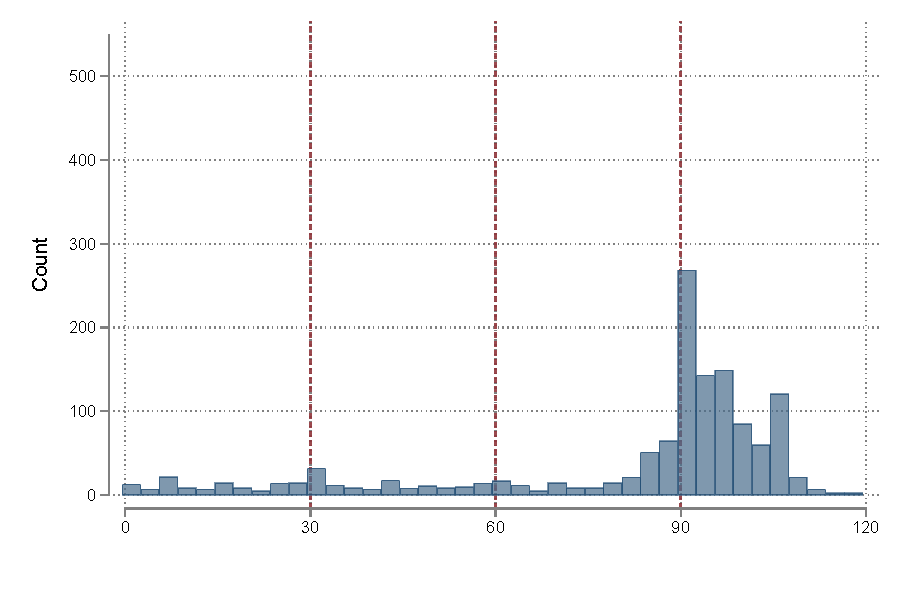
\includegraphics[width=\textwidth]{Figuras/hist_payments_sq.pdf}
    \end{center}
\end{figure}
\end{column}

\begin{column}{.33\textwidth}
    \begin{figure}[H]
    \caption{Forced commitment}
    \begin{center}
        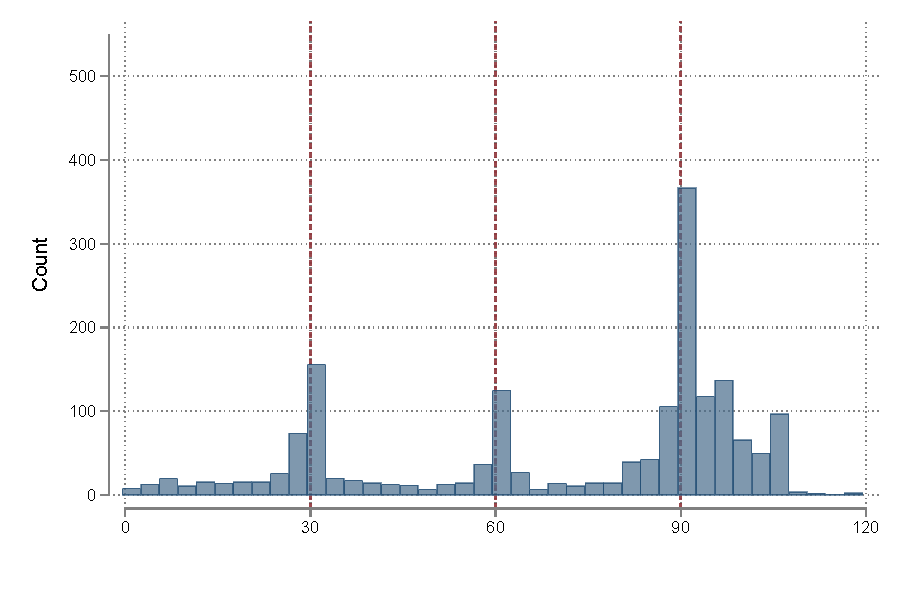
\includegraphics[width=\textwidth]{Figuras/hist_payments_fc.pdf}
    \end{center}
\end{figure}
\end{column}

\begin{column}{.33\textwidth}
    \begin{figure}[H]
    \caption{Choice commitment}
    \begin{center}
        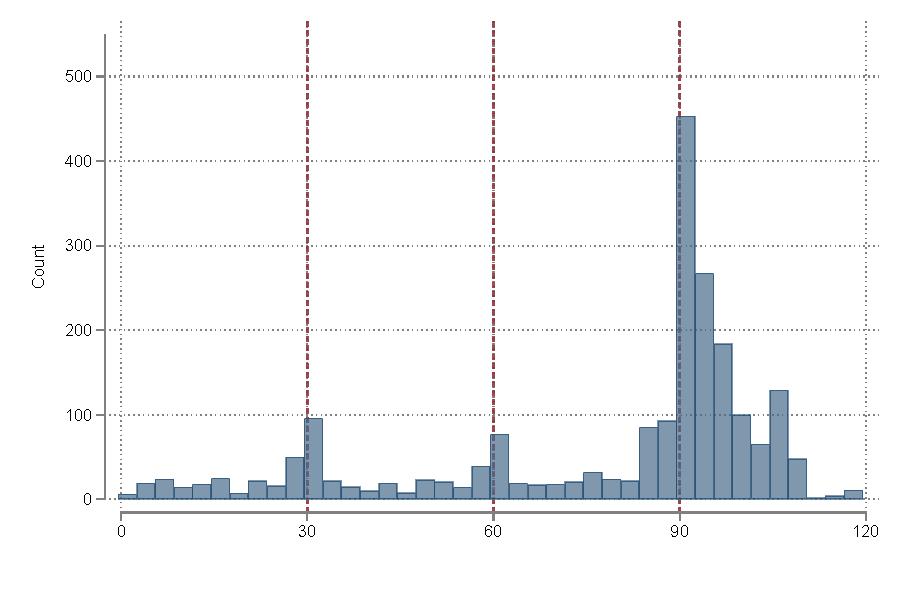
\includegraphics[width=\textwidth]{Figuras/hist_payments_cc.pdf}
    \end{center}
\end{figure}
\end{column}
\end{columns}


    
    \hyperlink{treatment_arms}{\beamerbutton{Back}}
\end{frame}



\begin{frame}{Distribution of financial cost (\$MXN)}
    \begin{figure}
     \centering
        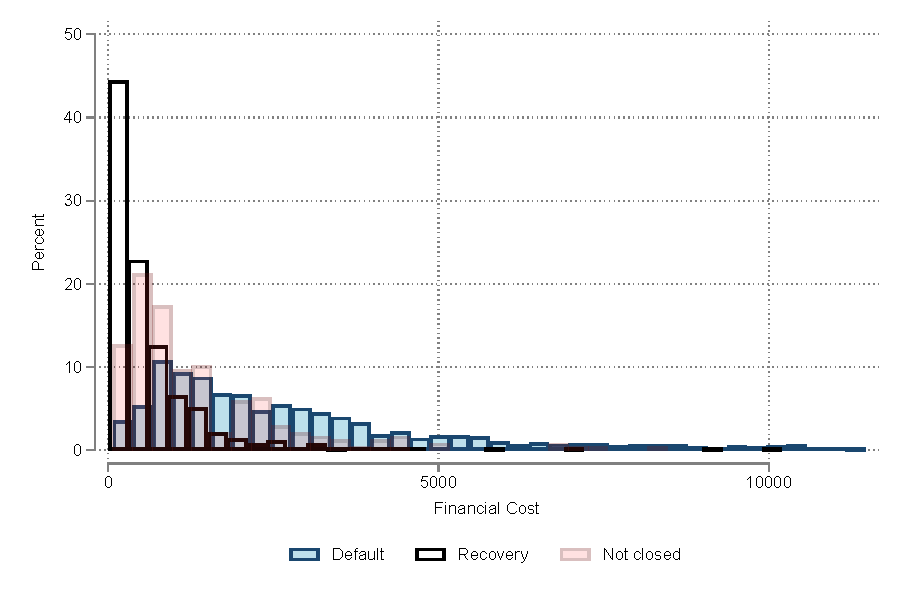
\includegraphics[width=.8\textwidth]{Figuras/hist_fc.pdf}
    \end{figure}
    
    \hyperlink{fc_outcome}{\beamerbutton{Back}}

\end{frame}


\begin{frame}{Appraiser FE}
\label{clerk_fe}
\begin{table}[H]
\begin{center}
\resizebox{0.95\textwidth}{!}{
\small{% Table generated by Excel2LaTeX from sheet 'clerk_fe'
\begin{tabular}{lcccccccc}
\toprule
      & \multicolumn{2}{c}{FC } &       & \multicolumn{2}{c}{Default} &       & \multicolumn{2}{c}{APR } \\
\cmidrule{2-3}\cmidrule{5-6}\cmidrule{8-9}      & (1)   & (2)   &       & (3)   & (4)   &       & (5)   & (6) \\
\midrule
\midrule
Forced commitment & -379.9*** & -363.9*** &       & -0.064*** & -0.063*** &       & -0.34*** & -0.34*** \\
      & (111.4) & (115.3) &       & (0.023) & (0.023) &       & (0.081) & (0.082) \\
Choice commitment & -78.8 & -116.9 &       & -0.023 & -0.022 &       & -0.10 & -0.10 \\
      & (114.5) & (117.7) &       & (0.021) & (0.021) &       & (0.074) & (0.075) \\
      &       &       &       &       &       &       &       &  \\
\midrule
Observations & 6304  & 6304  &       & 6304  & 6304  &       & 6304  & 6304 \\
R-squared & 0.007 & 0.018 &       & 0.013 & 0.025 &       & 0.011 & 0.020 \\
Appraiser FE &       & \checkmark &       &       & \checkmark &       &       & \checkmark \\
\bottomrule
\bottomrule
\end{tabular}%
}
}
\end{center}
 \scriptsize 
 
%\textit{Do file: } \texttt{clerk\_fe.do}
\end{table}
    \hyperlink{main_results}{\beamerbutton{Back}}

\end{frame}



\begin{frame}{Several definitions of cost}
\label{several_def_cost}
\begin{table}[H]
\caption{Effects on several definitions of cost}
\label{table_robustness_fc}
\begin{center}
\resizebox{0.95\textwidth}{!}{
\small{% Table generated by Excel2LaTeX from sheet 'fc_robustness_pres'
\begin{tabular}{lccccc}
\toprule
      & FC    & FC (subj.value) & FC +  tc & FC - interest & FC (subj.value) + tc - int \\
\midrule
      & (1)   & (2)   & (3)   & (4)   & (5) \\
\midrule
\midrule
Forced commitment & -379.7*** & -473.6*** & -383.4*** & -272.2** & -320.0** \\
      & (111.4) & (151.0) & (110.9) & (108.8) & (144.3) \\
Choice comitment & -84.9 & -104.0 & -78.6 & -79.8 & -72.9 \\
      & (114.6) & (153.8) & (114.3) & (114.2) & (149.0) \\
      &       &       &       &       &  \\
\midrule
Observations & 6304  & 6304  & 6304  & 6304  & 6304 \\
R-squared & 0.007 & 0.007 & 0.007 & 0.006 & 0.006 \\
Control Mean & 1851.0 & 2297.2 & 1934.7 & 1387.9 & 1834.9 \\
\bottomrule
\bottomrule
\end{tabular}%
}
}
\end{center}
 \scriptsize 
 
%\textit{Do file: } \texttt{fc\_robustness.do}
\end{table}
    \hyperlink{main_results}{\beamerbutton{Back}}

\end{frame}



\begin{frame}{Survival Graph}
   \label{interpolation_censoring_imp}

\begin{columns}
\begin{column}{.45\textwidth}

\begin{figure}[H]
    \begin{center}
    \caption{Ended}
        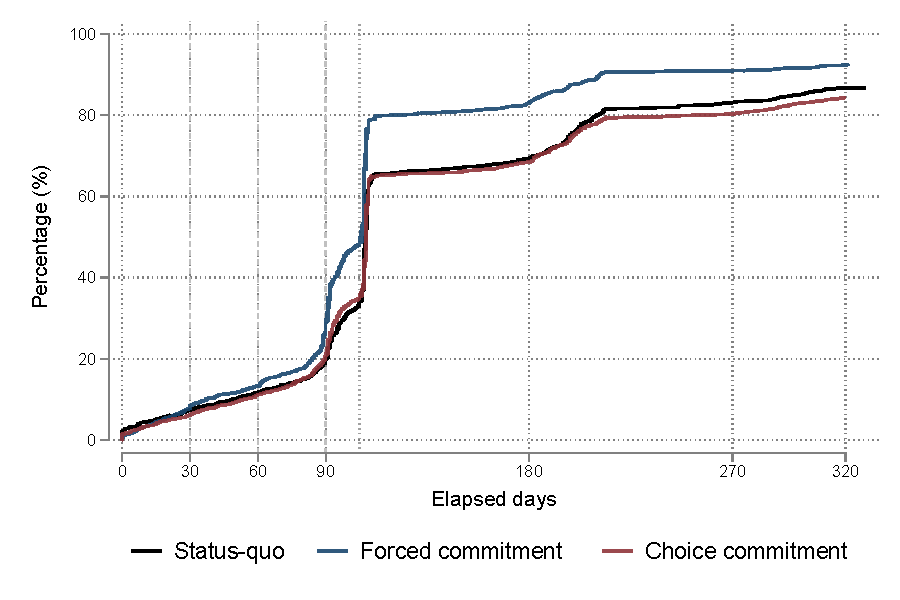
\includegraphics[width=1.1\textwidth]{Figuras/survival_graph_ended.pdf}
    \end{center}
    \end{figure}

    
    \end{column}
 
    
\begin{column}{.45\textwidth}

\begin{figure}[H]
    \begin{center}
    \caption{Recovery}
        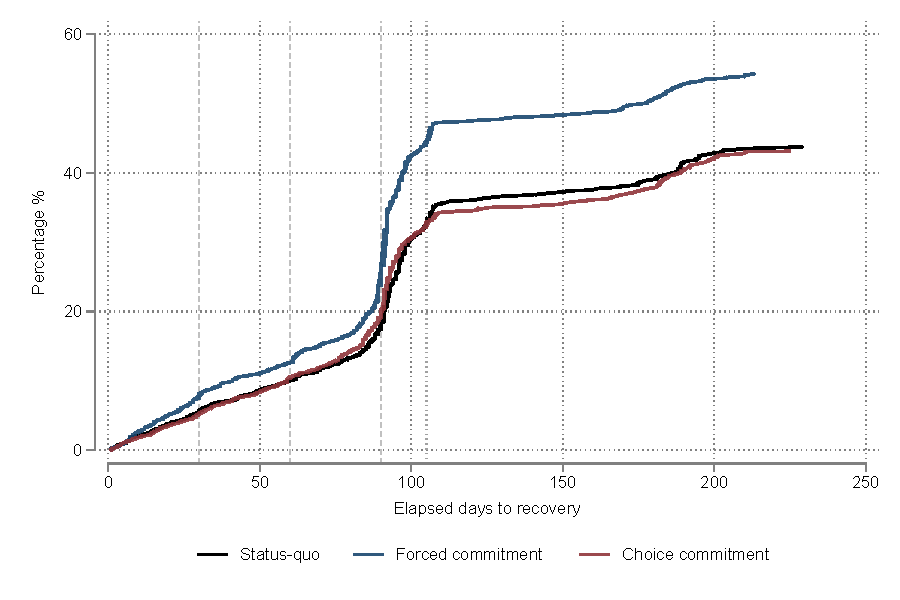
\includegraphics[width=1.1\textwidth]{Figuras/survival_graph_unpledge.pdf}
    \end{center}
    \end{figure}
 
    
    \end{column}    
    \end{columns}
\end{frame}


\begin{frame}{Censoring}
\label{censoring}
    \begin{table}[H]
\caption{Bounding censoring}
\label{bounding_censoring}
\begin{center}
\resizebox{0.9\textwidth}{!}{
\footnotesize{% Table generated by Excel2LaTeX from sheet 'censoring_imp_pres'
\begin{tabular}{lccccc}
\toprule
      & Control  = 0  & Control  = 0  & Control  = 1 & Control  = 1  & Prediction  \\
      & Forced arm = 0 & Forced arm = 1 & Forced arm = 0 & Forced arm = 1 & model \\
\midrule
      & \multicolumn{5}{c}{Financial Cost} \\
\midrule
      & (1)   & (2)   & (3)   & (4)   & (5) \\
\midrule
\midrule
Forced commitment  & -408.7*** & -226.5** & -804.2*** & -622.0*** & -525.3*** \\
      & (107.1) & (110.8) & (113.3) & (117.3) & (122.0) \\
      &       &       &       &       &  \\
\midrule
Observations & 3724  & 3724  & 3724  & 3724  & 3724 \\
R-sq  & 0.012 & 0.009 & 0.022 & 0.015 & 0.012 \\
Control Mean & 1898.5 & 1898.5 & 2272.4 & 2272.4 & 2073.6 \\
\midrule
\midrule
      &       &       &       &       &  \\
\midrule
      & \multicolumn{5}{c}{Default} \\
\midrule
\midrule
      & (6)   & (7)   & (8)   & (9)   & (10) \\
\midrule
\midrule
Forced commitment  & -0.063*** & 0.0089 & -0.21*** & -0.13*** & -0.12*** \\
      & (0.023) & (0.024) & (0.023) & (0.024) & (0.025) \\
      &       &       &       &       &  \\
\midrule
Observations & 3724  & 3724  & 3724  & 3724  & 6304 \\
R-sq  & 0.019 & 0.014 & 0.053 & 0.028 & 0.016 \\
Control Mean & 0.44  & 0.44  & 0.57  & 0.57  & 0.51 \\
\bottomrule
\bottomrule
\end{tabular}%
}
}
\end{center}
 \scriptsize 
%\textit{Do file: } \texttt{censoring_imp.do, censoring_imp_pr.do}
\end{table}


\end{frame}


\begin{frame}{Interpolation on bounding censoring}
    
\begin{figure}[H]
        \caption{Significance area for Default}
  
    \begin{center}
        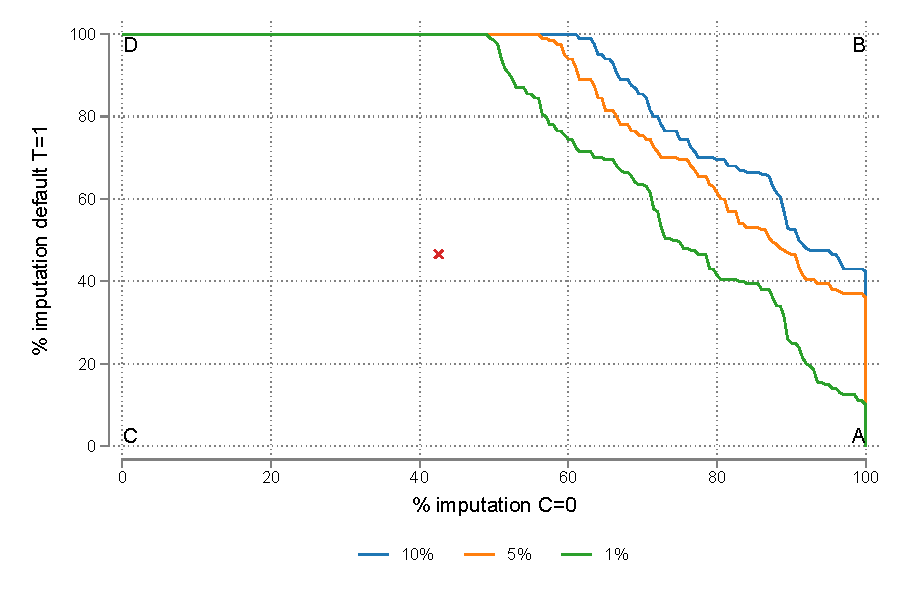
\includegraphics[width=0.75\textwidth]{Figuras/frontera_sig_def_imp.pdf}
    \end{center}
\end{figure}
 \hyperlink{main_results}{\beamerbutton{Back}}
\end{frame}



% \begin{frame}{Contract terms}

% \begin{figure}[H]
%      \caption{Contract Terms Summary}
%     \label{PaperSlip}
%     \begin{center}
%         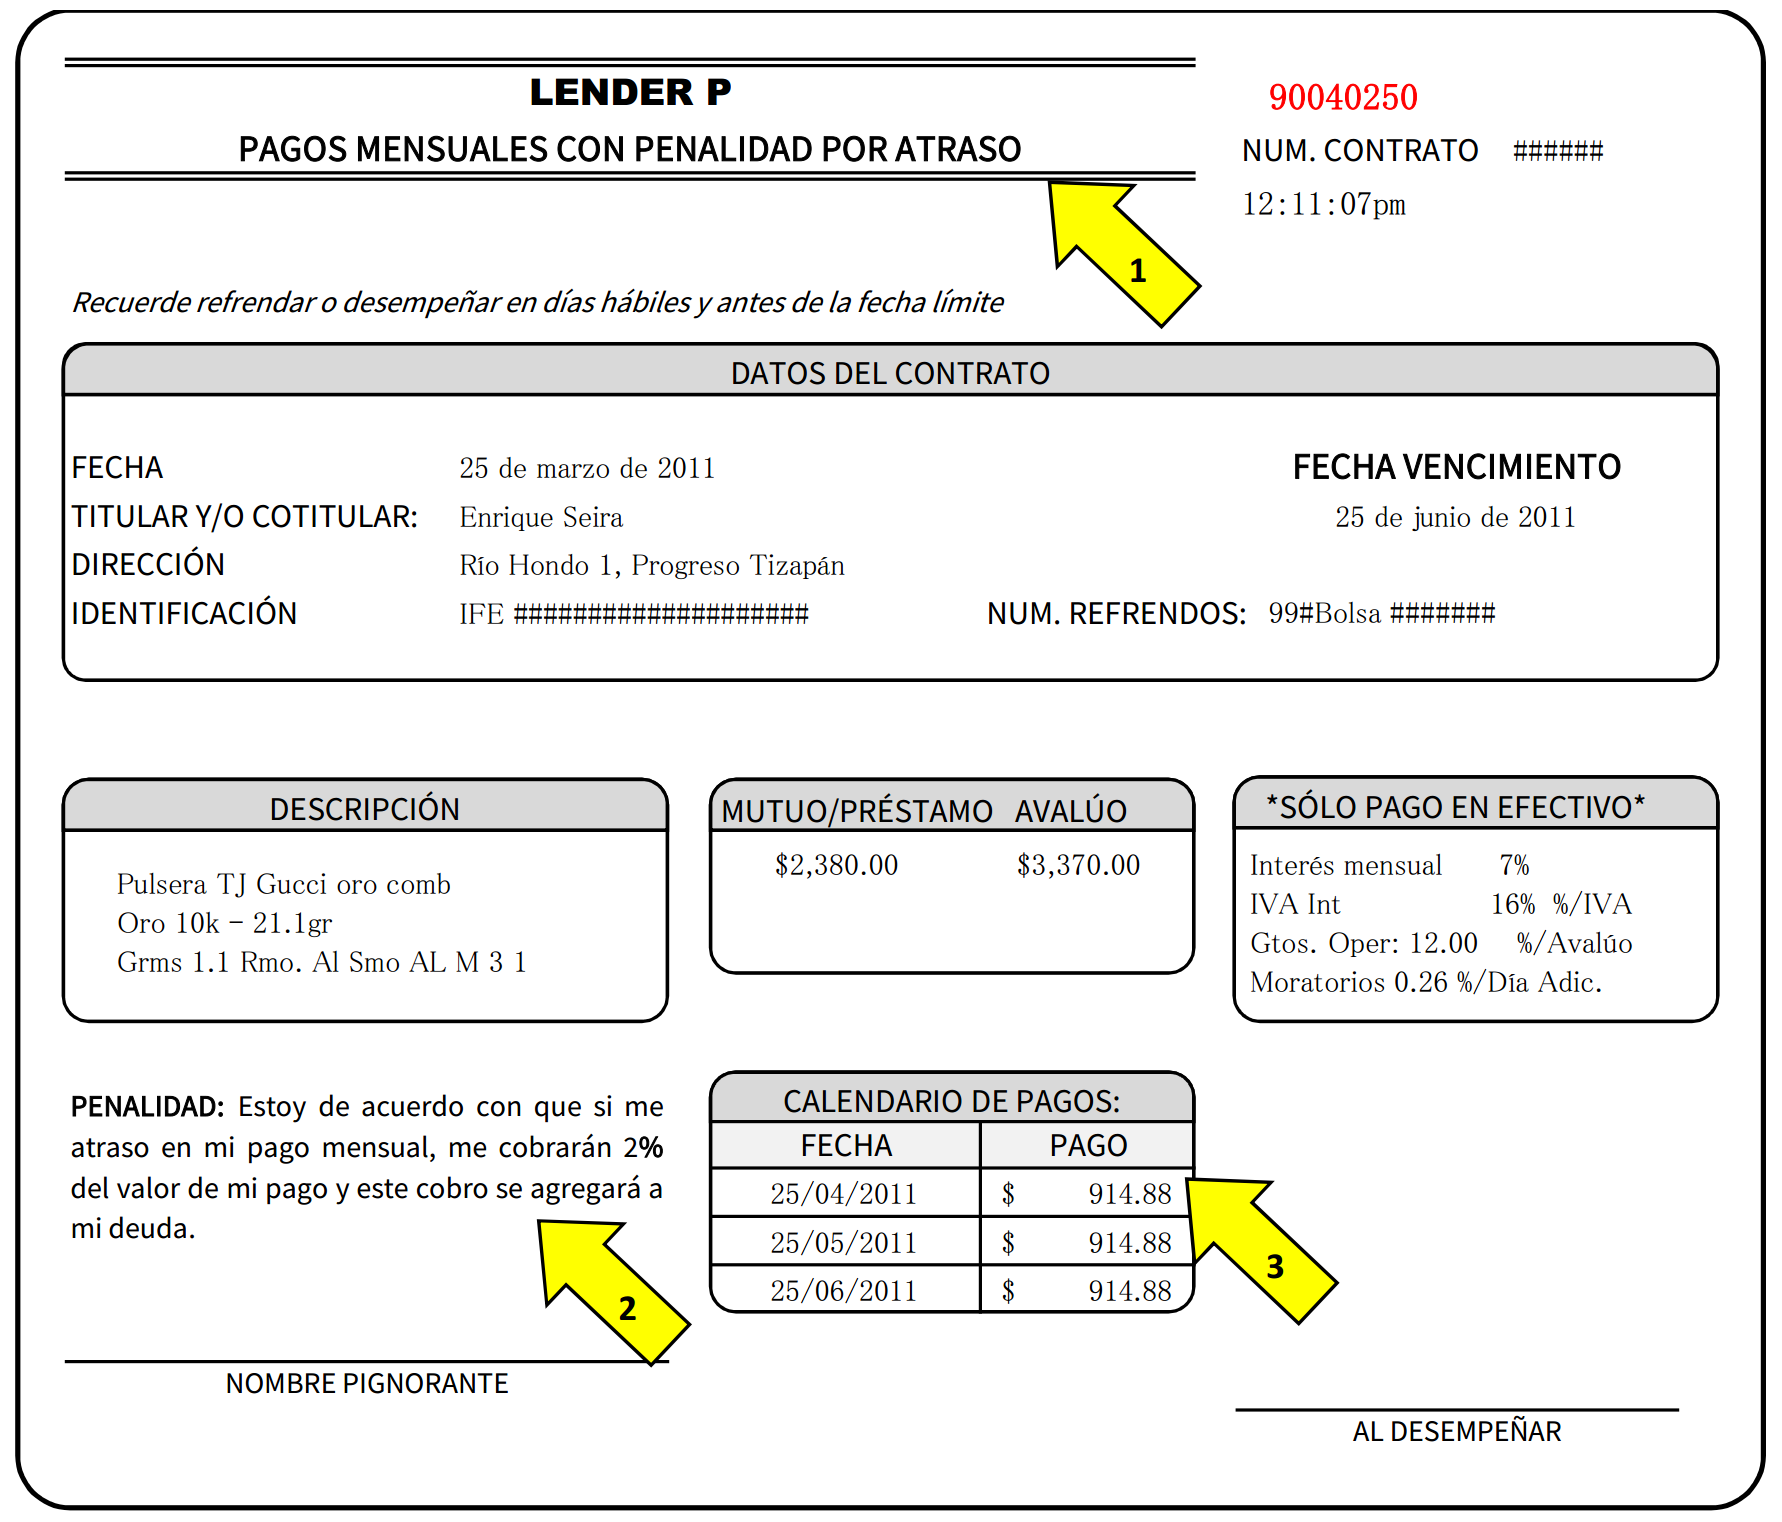
\includegraphics[width=0.65\textwidth]{Figuras/TicketLenderP.png}

%     \end{center}

% \end{figure}
% \end{frame}

\begin{frame}{Intermediate outcomes}
\label{mechanism_appendix}

\begin{table}[H]
\caption{Intermediate outcomes}
\begin{center}
\footnotesize{% Table generated by Excel2LaTeX from sheet 'mechanism_pres'
\begin{tabular}{lcc}
\toprule
      & \multicolumn{2}{c}{Panel A  : Speed of payment} \\
\cmidrule{2-3}      & Days to 1st payment & \% of payment in 1st visit \\
\midrule
\midrule
      & (1)   & (2) \\
\midrule
\midrule
Forced cmit & -13.8*** & 7.70*** \\
      & (1.61) & (2.78) \\
Choice cmit & -3.51** & -0.85 \\
      & (1.57) & (2.19) \\
      &       &  \\
\midrule
Observations & 4412  & 6304 \\
R-squared & 0.055 & 0.014 \\
Control Mean & 82.8  & 44.7 \\
\midrule
\midrule
      &       &  \\
\midrule
      & $\Pr($Recovery in 1st visit) & Loan duration (days) \\
\midrule
\midrule
      & (3)   & (4) \\
\midrule
\midrule
Forced cmit & 0.079*** & -27.9*** \\
      & (0.026) & (4.35) \\
Choice cmit & -0.010 & -0.18 \\
      & (0.022) & (4.33) \\
      &       &  \\
\midrule
Observations & 6304  & 6304 \\
R-squared & 0.016 & 0.054 \\
Control Mean & 0.30  & 136.6 \\
\bottomrule
\bottomrule
\end{tabular}%
}
\end{center}
\end{table}
\vfill
\hyperlink{intermediate_outcomes}{\beamerbutton{Back}}
\end{frame}

\begin{frame}{Intermediate outcomes}

\begin{table}[H]
\caption{Intermediate outcomes}
\begin{center}
\footnotesize{% Table generated by Excel2LaTeX from sheet 'mechanism_pres'
\begin{tabular}{lccc}
\toprule
      & \multicolumn{3}{c}{Panel B  : Variables related to default} \\
\cmidrule{2-4}      & $\Pr($+ payment \& default) & \% of pay $|$ def  & $\Pr($Selling pawn $|$ def) \\
\midrule
\midrule
      & (5)   & (6)   & (7) \\
\midrule
\midrule
Forced cmit & -0.070*** & -3.96*** & 0.14*** \\
      & (0.015) & (1.27) & (0.034) \\
Choice cmit & -0.028** & -2.11** & 0.053* \\
      & (0.014) & (1.04) & (0.029) \\
      &       &       &  \\
\midrule
Observations & 6304  & 2486  & 2486 \\
R-squared & 0.011 & 0.023 & 0.033 \\
Control Mean & 0.12  & 9.59  & 0.71 \\
\bottomrule
\bottomrule
\end{tabular}%
}
\end{center}
\end{table}
\vfill
\hyperlink{intermediate_outcomes}{\beamerbutton{Back}}
\end{frame}


\begin{frame}{Intermediate outcomes}

    \begin{table}[H]
\caption{Intermediate outcomes}
\begin{center}
\footnotesize{% Table generated by Excel2LaTeX from sheet 'mechanism_pres'
\begin{tabular}{lcc}
\toprule
      & \multicolumn{2}{c}{Panel C  : Visit variables} \\
\cmidrule{2-3}      & \# of visits & \# of visits $|$ def \\
\midrule
\midrule
      & (8)   & (9) \\
\midrule
\midrule
Forced cmit & -0.031 & -0.19*** \\
      & (0.049) & (0.049) \\
Choice cmit & 0.085 & -0.090** \\
      & (0.053) & (0.042) \\
      &       &  \\
\midrule
Observations & 6304  & 2486 \\
R-squared & 0.022 & 0.026 \\
Control Mean & 1.14  & 0.39 \\
\bottomrule
\bottomrule
\end{tabular}%
}
\end{center}
\end{table}
\vfill
\hyperlink{intermediate_outcomes}{\beamerbutton{Back}}
\end{frame}






\begin{frame}{Bounding Individual Treatment Effects}
\label{fan_park_bounds}    

\begin{figure}[H]
    \caption{Fan \& Park bounds for benefit in effective FC }
    
    \begin{center}
        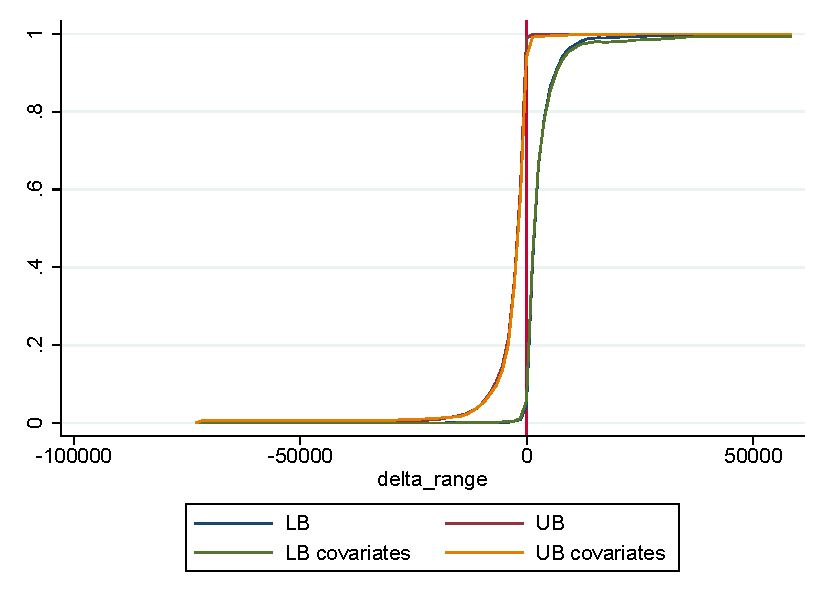
\includegraphics[width=0.75\textwidth]{Figuras/fan_park_bounds_fc_admin.pdf}
    \end{center}
   
\end{figure}
 \hyperlink{choice_hte}{\beamerbutton{Back}}
\end{frame}


 
 
\begin{frame}{Identification of treatment parameters}
\label{identification_randomized_choice}
\begin{equation*}
    Y_i = \mathbbm{1}(Z_i =0) Y_{i0} + \mathbbm{1}(Z_i = 1)  Y_{i1}  + \mathbbm{1}(Z_i = 2) \left[(1 - C_i) Y_{i0} + C_i Y_{i1} \right].
\label{eq:potentialOutcomes}
\end{equation*}

    Viewing $Z_i$ as an instrumental variable, the randomized choice design can be interpreted as a \emph{pair} of RCTs, each subject to one-sided non-compliance. \\
    \begin{itemize}
        \item The first of these compares $Z_i=0$ to $Z_i = 2$.  This setting is identical to a ``randomized encouragement'' design in which treatment is only available to those who are encouraged: $Z_i = 2$. Under this interpretation, those with $C_i = 1$ are ``the compliers'' and it follows that 
\begin{equation*}
\frac{\mathbbm{E}(Y_i|Z_i=2) - \mathbbm{E}(Y_i|Z_i =0)}{\mathbbm{E}(D_i|Z_i=2)-\mathbbm{E}(D_i|Z_i=0)}  = \mathbbm{E}(Y_{i1} - Y_{i0}|C_i = 1)
\label{eq:ToT}
\end{equation*}

\item The second considers $Z_i = 1$ to be the ``encouragement'' and compare the outcomes for these individuals to those with $Z_i = 2$.
\begin{equation*}
\frac{\mathbbm{E}(Y_i|Z_i=1) - \mathbbm{E}(Y_i|Z_i =2)}{\mathbbm{E}(D_i|Z_i=1)-\mathbbm{E}(D_i|Z_i=2)}  = \mathbbm{E}(Y_{i1} - Y_{i0} | C_i = 0)
\label{eq:TuT}
\end{equation*}


\item Because non-compliance is one-sided only, LATE=ToT in one case (since treated=compliers+always takers, but there are no always takers, as they cannot take without being assigned) and LATE=TuT in the other.

\end{itemize}
\hyperlink{cc_design}{\beamerbutton{Back}}


\end{frame}





\end{document}






